\documentclass[manuscript,screen,review]{acmart}
\acmJournal{TECS}
\setcopyright{none}
\settopmatter{printacmref=false}
\usepackage{tikz}
\usetikzlibrary{arrows.meta,positioning,calc,fit,backgrounds}
\usepackage{pgfplots}
\pgfplotsset{compat=1.18}
\usepackage{tabularx}
\graphicspath{{figures/}{../figures/}}
\newcommand{\protset}{\mathcal{P}}
\newcommand{\risk}{\mathcal{R}}
\newcommand{\E}{\mathbb{E}}
\newcommand{\Prob}{\mathbb{P}}
\newcommand{\bits}{\mathcal{B}}
\newcommand{\code}[1]{\texttt{#1}}
\newcommand{\clip}{\operatorname{clip}}
\definecolor{nsnavy}{HTML}{18354A}
\definecolor{nsteal}{HTML}{087E8B}
\definecolor{nsgold}{HTML}{BC771B}
\definecolor{nspale}{HTML}{EFF4F6}
% ---------------------------------------------------------------- draft v2 (rate-aware) placeholders
% \TBD{...}            a number or statement that waits for a Run R result
% \Branch{rule}{if the rule holds}{if it fails}   both versions are printed until the result picks one
% \RuleHolds{R1}       after a result: \setbranch{R1}{holds} or {fails} prints only that version
\newcommand{\TBD}[1]{\textcolor{red}{\textbf{[TBD:} #1\textbf{]}}}
\newcommand{\TBDcite}[1]{\textcolor{red}{[cite: #1]}}
\newcommand{\TBDfig}[2]{\fbox{\parbox[c][#1][c]{.95\linewidth}{\centering\textcolor{red}{\textbf{Figure placeholder:} #2}}}}
\makeatletter
\newcommand{\setbranch}[2]{\expandafter\def\csname branch@#1\endcsname{#2}}
\newcommand{\Branch}[3]{%
  \@ifundefined{branch@#1}{%
    {\color{nsteal}[\textbf{if #1 holds:} #2]}~{\color{nsgold}[\textbf{if #1 fails:} #3]}}{%
    \expandafter\ifx\csname branch@#1\endcsname\branch@holdsword #2\else #3\fi}}
\def\branch@holdsword{holds}
\makeatother
\newcommand{\rhos}{\rho}

\title[Which Bits to Protect Depends on the Fault Rate]{Which Stored Bits to Protect Depends on the Fault Rate: Predicting the Switch and Assigning Protection in INT8 Neural Networks}
\author{Manuel Blanco Valent\'in}
\affiliation{\department{Electrical and Computer Engineering}\institution{Northwestern University}\city{Evanston}\state{Illinois}\country{USA}}
\author{Houxuan Guo}
\affiliation{\department{Electrical and Computer Engineering}\institution{Northwestern University}\city{Evanston}\state{Illinois}\country{USA}}
\author{Xiuyuan He}
\affiliation{\department{Electrical and Computer Engineering}\institution{Northwestern University}\city{Evanston}\state{Illinois}\country{USA}}
\author{Seda Ogrenci}
\affiliation{\department{Electrical and Computer Engineering}\institution{Northwestern University}\city{Evanston}\state{Illinois}\country{USA}}
\renewcommand{\shortauthors}{Blanco Valent\'in et al.}
\ccsdesc[500]{Computer systems organization~Reliability}
\ccsdesc[300]{Computer systems organization~Embedded systems}
\ccsdesc[300]{Computing methodologies~Neural networks}
\keywords{quantized neural networks, fault injection, selective protection, triple modular redundancy, error-correcting codes, stored-bit faults, reliability}

% Draft v2 (rate-aware). Results of Run R are placeholders. To fix a branch once its result is in, uncomment:
\setbranch{R1}{holds}   % Stage 1 confirmed (RUN_R_STAGE1_RESULTS_2026-11-12.md)
% \setbranch{R2}{holds}   % Stage 2, rate-aware assignment never far behind (R2a and R2b)
% \setbranch{R3a}{holds}  % Stage 3a, residual curves match simulation
% \setbranch{R3b}{holds}  % Stage 3b, per-bit choice of scheme helps
\begin{document}
\begin{abstract}
Selective protection of neural-network weights spends a limited budget of redundancy on the stored bits that matter most, and almost every proposal ranks the bits once and protects the top of the list. We show that which bits are worth protecting depends on the bit-error probability $p$, and explain why. Writing the expected loss of a faulty model as the loss at the average faulty weights plus a curvature-weighted variance gives a cost with one term per bit, proportional to $p$, and one term per pair of bits, proportional to $p^2$. A fixed ranking is optimal only while the first dominates: at sparse fault rates the bits worth protecting are those whose flips raise the loss on average, and at dense rates those whose flips together would push the weights in one direction. The same expression gives the rate at which the preferred ranking switches, from calibration data alone. \Branch{R1}{On nine ResNet-8 checkpoints, with every prediction fixed before the faults were drawn, the predicted switch agreed with the measured one within a factor of 1.5 on every checkpoint and was about 12\% late on average, and the better ranking matched the prediction in every statistically resolved comparison away from the switch.}{On nine ResNet-8 checkpoints the predicted switch did not meet the location criterion fixed in advance \TBD{measured/predicted ratio}, although \TBD{R1a/R1b outcome}.} Because protection is rarely perfect, the cost uses the residual error probability of each mechanism (triplication, five copies, SEC-DED codes and checksum correction), so mechanisms and bits are chosen together. \Branch{R2}{An assignment that minimizes this cost for the given $p$ is never more than half an accuracy point behind the best of nine rankings and searches at any rate where the model is usable, while every static ranking falls behind somewhere \TBD{largest gaps}.}{An assignment that minimizes this cost \TBD{Stage 2 outcome}.} Across six frozen INT8 models, from MLPerf Tiny networks to a 0.6-billion-parameter language model, significance-first protection tolerates about a third of the bit-error probability of gradient-based masks on four models. Protection is logical suppression with idealized voters and decoders; no hardware-cost or radiation-rate claim is made.
\end{abstract}
\maketitle
\section{Introduction}\label{sec:introduction}
Neural-network accelerators at the edge keep their weights in on-chip storage for the whole deployment, so a corrupted weight bit persists across inferences until it is rewritten. Where faults are expected, as in the radiation-hard front-end ASICs of particle detectors, every register is triplicated~\cite{cummings2023econd,diguglielmo2021reconfigurable}. Elsewhere that cost is often unaffordable, which makes selective protection attractive: spend a limited budget on the bits that matter most~\cite{libano2019selective,garciabertoa2023selective,nazari2024fortune,guo2025inpixel}. Almost every proposal does this with a ranking computed once: bit significance, a gradient or a Hessian score~\cite{weng2024fkeras}, or a measured single-flip vulnerability~\cite{tyagi2023thales}. The ranking is then protected from the top down at whatever budget is available.

A fixed ranking assumes that the value of protecting a bit does not depend on what else fails. It does. Protecting a bit removes its effect in a network that already carries the faults of every other unprotected bit, so the value of protection depends on the bit-error probability $p$ and on the rest of the mask, a fact long known in reliability theory~\cite{birnbaum1969importance,rausand2004system}. We found that it matters in practice. Two gradient rankings that differ only in whether they keep the sign of a flip's predicted effect trade places on all nine ResNet-8 checkpoints we studied when both are built from 1,024 calibration inputs: the one that protects loss-increasing flips is ahead by up to 1.6 accuracy points at $p=10^{-3}$ and behind by up to 18 at $10^{-2}$ (Appendix~\ref{app:calibration}). On a language model the same ranking is worse than no protection at all (Appendix~\ref{app:harm}). These observations raise three questions that a designer needs answered. Why does the preferred ranking change with the fault rate? Can the change be predicted before any fault is injected? And can protection be assigned so that it is never far from the best choice, whatever the rate and whatever mechanism provides the protection?

This paper answers them with an expression for the expected loss of a faulty model and a set of tests designed around its predictions.

\paragraph{The expected loss of a faulty model.} Independent stored-bit faults move every weight by a random amount. Expanding the loss to second order around the \emph{average} faulty weights, instead of around the clean ones, splits the expected loss into the loss at those average weights and a curvature-weighted variance (Section~\ref{sec:theory}). Expanded in $p$, the first part contributes one term per bit, which is proportional to $p$ and keeps the sign of a flip's effect, and one term per pair of bits, which is proportional to $p^2$ and penalizes unprotected flips that push the weights in the same direction. A ranking is optimal only while the per-bit term dominates. The pairwise term takes over at a rate $p^*$ that depends on how far the model is from a minimum of its loss and that can be computed from calibration data.

\paragraph{Imperfect protection.} Real mechanisms do not suppress faults; they lower their probability. A triplicated bit is still wrong with probability $3p^2-2p^3$, a bit in a SEC-DED word when another bit of the word also flips, and a weight under checksum correction when another weight of its group is faulty, or when the decoder repairs the wrong weight. Each mechanism therefore has a residual error curve $\rho_s(p)$ (Section~\ref{sec:fault}), and the same expected-loss expression accepts a different residual rate for every bit. Choosing which bits to protect and how to protect them becomes one problem.

\paragraph{Contributions.}
\begin{itemize}
\item \textbf{An explanation of why the preferred ranking depends on the fault rate}, from a second-order expansion of the expected loss around the average faulty weights, and a prediction of the rate $p^*$ at which it switches, computed from calibration data without fault injection (Section~\ref{sec:theory}). \Branch{R1}{The prediction was fixed before the faults were drawn and \TBD{agrees with the measured switch within a factor of R1c} on nine ResNet-8 checkpoints and eight budgets (Section~\ref{sec:switch}).}{It was tested with every prediction fixed before the faults were drawn; \TBD{what held and what did not} (Section~\ref{sec:switch}).}
\item \textbf{Residual error curves for triplication, five copies, SEC-DED codes and checksum correction}, including the wrong repairs of checksum decoders, placed in the same cost (Sections~\ref{sec:fault} and~\ref{sec:theory}). \Branch{R3a}{Each curve matches a bit-level simulation of its mechanism \TBD{R3a}.}{\TBD{which curves did not match simulation}.}
\item \textbf{A rate-aware protection assignment} that minimizes the cost for a given $p$ and storage budget by budget-preserving swaps, with an optional Monte Carlo correction for the large jumps of sign and high-order bits (Section~\ref{sec:method}). \Branch{R2}{On ResNet-8 it is the only tested mask that is never more than half an accuracy point behind the best one at any rate where the model is usable \TBD{largest gap}; the absolute- and positive-gradient rankings each fall behind by \TBD{gaps} somewhere.}{\TBD{Stage 2 outcome, stated as measured}.} \Branch{R3b}{Letting it choose between triplication and five copies per bit improves on ranked triplication by \TBD{R3b}.}{Choosing the mechanism per bit did not improve on ranked triplication \TBD{R3b}.}
\item \textbf{A paired evaluation of seven static rankings on six frozen INT8 models}, from MLPerf Tiny networks to a 0.6-billion-parameter language model, which provides the evidence base (Section~\ref{sec:static} and Appendix~\ref{app:static}). Significance-first protection keeps four of the six models useful only up to about a third of the bit-error probability tolerated by the per-example absolute-gradient mask, and falls 9 to 34 points behind it on every ResNet-8 checkpoint at a moderate fault rate.
\end{itemize}

The study is software-only. Faults are exact XOR flips of stored INT8 weight codes, outcomes come from the quantized executables, and voters and decoders are idealized. We do not measure the area, power or latency of any mechanism, and logical $p$ is not a radiation exposure rate. Our earlier design flow connected susceptibility ranking to selective redundancy and hardware synthesis~\cite{guo2025inpixel}; none of that hardware evidence is reused here.

\section{Related Work and Scope}\label{sec:related}
\paragraph{Sensitivity ranking and fault discovery.} FKeras ranks weights by a projection onto leading Hessian eigenvectors and orders bits by significance tier~\cite{weng2024fkeras}. Its authors compare random, significance, gradient and Hessian orderings against single-bit oracles and note that a strict tier-first order is not ideal; for one autoencoder they report that protecting the bits found sensitive to single flips also removed the errors of simultaneous flips. PrioriFI quantifies the exceptions to bit-level monotonicity and reorders fault-injection campaigns by observed damage~\cite{weng2026priorifi}, and EISFINN uses attribution to drive importance-sampled campaigns~\cite{colucci2024eisfinn}. Thales defines a DNN-specific architectural vulnerability factor, the expected accuracy given one transient fault in a flip-flop, and assumes that SRAM and DRAM are protected by ECC or parity~\cite{tyagi2023thales}. These works rank bits or schedule injections. They do not compare equal-budget protection masks under a common multi-fault law, and our setting is the complement of Thales: many persistent faults in weight storage that is not rewritten. Appendix~\ref{app:search} adapts Thales and HarDNN to stored-bit protection.

\paragraph{Protection mechanisms and allocation.} Selective hardening and channel-level TMR predate this study~\cite{libano2019selective,garciabertoa2023selective}. FORTUNE triplicates each weight's most significant bit alongside quantization~\cite{nazari2024fortune}. HarDNN and its follow-up rank the feature maps of a CNN by their vulnerability to transient errors in computation, by injected loss change or by cheaper heuristics of which the mean gradient magnitude was the most accurate, and duplicate the filters of the most vulnerable maps; they too assume protected storage~\cite{mahmoud2020hardnn,mahmoud2021optimizing}. Ranger restricts intermediate values to their fault-free ranges~\cite{chen2021ranger}, a bound already implied by the fully integer arithmetic executed here. Algorithm-based fault tolerance (ABFT) uses checksums to detect, and for few errors per group correct, faults in a matrix product~\cite{alyamani2001abft,zhao2021ftcnn}; it recovers transient errors by recomputation, which does not remove a persistent fault in a stored weight. Section~\ref{sec:correction} compares TMR of ranked bits with SEC-DED codes and ABFT checksum correction under one fault model. Progressive Bit Search, DeepHammer and FlipLLM search for small damaging bit sets~\cite{rakin2019bitflip,yao2020deephammer,khalil2026flipllm}, which differs from minimizing expected risk under random faults. Reinforcement learning has been used to allocate protection, learning layer-wise bit-position masks~\cite{su2025rl} or selective-ECC allocations compared with rule-based ones at matched cost~\cite{alobaidi2026selectiveecc}. No matched implementation of these allocators on our models is available, so we claim no superiority over them; Section~\ref{sec:discussion} reports a relaxed per-bit optimizer, the closest relative we implemented. Training for robustness to random bit errors at a given BER~\cite{stutz2021biterror} is complementary; we protect a fixed model.

\paragraph{Protection value in reliability theory.} Birnbaum's importance is the partial derivative of system reliability with respect to one component's reliability, and the improvement potential is that importance multiplied by the component's failure probability~\cite{birnbaum1969importance,rausand2004system}. Both depend on the failure probabilities of the other components, so importance rankings are not fixed properties of a system. Section~\ref{sec:allocation} restates this for bit protection; we claim no novelty for the identity, only for measuring what it implies in quantized networks.

\section{Fault Model and Protection Mechanisms}\label{sec:fault}
The evaluation freezes a trained model, its numerical execution and its task data; builds protection assignments from calibration data; and compares them under common random faults (Fig.~\ref{fig:workflow}). All clean and faulted outcomes come from the quantized executable itself, not from the differentiable companion model used to compute gradients. NetSuRF is the software implementation of this workflow; it is not a ranking in the comparison.

\begin{figure}[t]
\centering% Vector adaptation of the original NetSuRF three-panel workflow.
% The historical visual structure is retained; all stages describe software evidence.
\begingroup%
\definecolor{flowbrown}{HTML}{693E25}%
\definecolor{flowcream}{HTML}{FAF6ED}%
\definecolor{flowgreen}{HTML}{EEF3D7}%
\definecolor{flowolive}{HTML}{84944B}%
\definecolor{flowred}{HTML}{B74232}%
\definecolor{flowink}{HTML}{343A3C}%
\resizebox{\linewidth}{!}{%
\begin{tikzpicture}[
  font=\sffamily\fontsize{8}{10}\selectfont,
  text=flowink, >=Stealth,
  edge/.style={->,draw=flowbrown,line width=.75pt},
  transfer/.style={->,draw=flowred,line width=1.15pt},
  group/.style={draw=flowbrown,fill=flowgreen,rounded corners=5pt,
                dashed,line width=.75pt},
  label/.style={align=center,font=\sffamily\bfseries\fontsize{8.3}{10}\selectfont},
  detail/.style={align=center,font=\sffamily\fontsize{7.7}{9.6}\selectfont}]

% Three familiar framed panels and brown stage headers.
\foreach \x in {0,4.6,9.2}{
  \draw[draw=flowbrown,fill=flowcream,line width=.9pt]
    (\x,0) rectangle +(4.4,5.9);
  \fill[flowbrown] (\x,5.12) rectangle +(4.4,.78);
}
\node[align=center,text=white,font=\sffamily\bfseries\fontsize{9.5}{11.5}\selectfont]
  at (2.2,5.51) {1. Frozen network\\and inputs};
\node[align=center,text=white,font=\sffamily\bfseries\fontsize{9.5}{11.5}\selectfont]
  at (6.8,5.51) {2. Stored-bit analysis\\and allocation};
\node[align=center,text=white,font=\sffamily\bfseries\fontsize{9.5}{11.5}\selectfont]
  at (11.4,5.51) {3. Paired reliability\\evaluation};

% Panel 1: immutable model and partition documents.
\draw[draw=flowolive,fill=white,line width=.8pt]
  (.35,3.35)--(.35,4.77)--(1.91,4.77)--(2.11,4.57)
  --(2.11,3.35)--cycle;
\draw[draw=flowolive,line width=.6pt]
  (1.91,4.77)--(1.91,4.57)--(2.11,4.57);
\node[label] at (1.23,4.31) {Frozen INT8\\checkpoint};
\node[detail] at (1.23,3.70) {Stored codes\\Scale / hash};
\draw[draw=flowolive,fill=white,line width=.8pt]
  (2.32,3.35)--(2.32,4.77)--(3.86,4.77)--(4.06,4.57)
  --(4.06,3.35)--cycle;
\draw[draw=flowolive,line width=.6pt]
  (3.86,4.77)--(3.86,4.57)--(4.06,4.57);
\node[label] at (3.19,4.31) {Task inputs};
\node[detail] at (3.19,3.80) {Calibration\\Evaluation};
\draw[group] (.30,.72) rectangle (4.10,2.91);
\node[label,text=flowbrown] at (2.20,2.61) {Verified frozen executable};
\draw[edge] (1.23,3.35)--(1.23,2.91);
\draw[edge] (3.19,3.35)--(3.19,2.91);
% Compact network motif, not a claim about a particular architecture.
\foreach \ya in {1.40,2.04}{
  \foreach \yb in {1.23,1.72,2.21}{
    \draw[flowbrown!45,line width=.45pt] (.65,\ya)--(1.10,\yb);
  }
}
\foreach \ya in {1.23,1.72,2.21}{
  \foreach \yb in {1.40,2.04}{
    \draw[flowbrown!45,line width=.45pt] (1.10,\ya)--(1.55,\yb);
  }
}
\foreach \x/\y in {.65/1.40,.65/2.04,1.10/1.23,1.10/1.72,1.10/2.21,1.55/1.40,1.55/2.04}{
  \filldraw[fill=white,draw=flowbrown,line width=.6pt] (\x,\y) circle (.075);
}
\node[detail,text width=2.10cm] at (2.91,1.73)
  {Exact model bytes\\Pinned backend\\Clean reference};
\node[detail,text=flowbrown] at (2.20,.34) {No retraining or model substitution};

% Panel 2: bit-table stack, calibration group, and sealed-mask motif.
\draw[draw=flowolive,fill=white,line width=.6pt]
  (5.02,3.48) rectangle (6.83,4.88);
\draw[draw=flowolive,fill=white,line width=.6pt]
  (4.94,3.40) rectangle (6.75,4.80);
\draw[draw=flowolive,fill=white,line width=.8pt]
  (4.86,3.32) rectangle (6.67,4.72);
\node[label] at (5.765,4.34) {Bit identities};
\node[detail] at (5.765,3.77) {Tensor / word\\Bit / XOR jump};
\node[label,text=flowbrown] at (7.85,4.70) {Fixed mask $P$};
\foreach \x in {0,...,3}{
  \foreach \y in {0,1}{
    \draw[draw=flowbrown!70,fill=white,line width=.55pt]
      (7.13+\x*.36,3.63+\y*.36) rectangle +(0.36,.36);
  }
}
\foreach \x/\y in {0/1,1/1,2/0}{
  \fill[flowolive!75] (7.13+\x*.36+.025,3.63+\y*.36+.025)
    rectangle +(0.31,.31);
}
\node[detail] at (7.85,3.36) {$|P|=B$};
\draw[group] (4.90,.72) rectangle (8.70,2.91);
\node[label,text=flowbrown] at (6.80,2.60) {Calibrate scores; order bits};
\node[detail] at (6.80,2.12) {Significance $\cdot$ jump $\cdot$ gradients};
\node[detail] at (6.80,1.73) {Published-form FKeras (TFLite)};
\node[label,text=flowred] at (6.80,1.13) {Choose budget; freeze mask};
\draw[edge] (5.765,3.32)--(5.765,2.91);
\draw[edge] (7.85,2.91)--(7.85,3.14);
\draw[transfer] (4.10,1.73)--(4.90,1.73);
\node[detail,text=flowbrown] at (6.80,.34) {Construction data only};

% Panel 3: same proposed field, exact suppressed XOR, inference, and outputs.
\draw[group] (9.50,2.30) rectangle (13.30,4.82);
\node[label,text=flowbrown] at (11.40,4.48) {Shared Bernoulli field $Z$};
\node[detail] at (11.40,4.03) {Suppress $P$; apply XOR on $Z\setminus P$};
\draw[transfer] (8.70,4.03)--(9.50,4.03);
\draw[edge] (11.40,3.80)--(11.40,3.58);
\draw[draw=flowbrown!75,fill=white,rounded corners=2pt,line width=.65pt]
  (9.74,2.56) rectangle (13.06,3.56);
\node[label] at (11.40,3.25) {Quantized inference};
\node[detail] at (11.40,2.83) {Held-out inputs; restore};
% Document motif for task measurements.
\draw[draw=flowolive,fill=white,line width=.55pt]
  (9.61,.48) rectangle (11.40,1.91);
\draw[draw=flowolive,fill=white,line width=.75pt]
  (9.53,.40) rectangle (11.32,1.83);
\node[label,text=flowbrown] at (10.425,1.55) {Task results};
\node[detail,font=\sffamily\fontsize{7.3}{8.5}\selectfont] at (10.425,.95)
  {CE / NLL\\Accuracy\\File ROC-AUC};
\draw[edge] (11.40,2.30)--(11.40,2.10)--(10.425,2.10)--(10.425,1.91);
\draw[edge] (11.40,2.10)--(12.36,2.10)--(12.36,1.91);
% Small illustrative chart: the actual measured curves appear in the results.
\draw[draw=flowbrown,line width=.7pt] (11.75,.74)--(11.75,1.78);
\draw[draw=flowbrown,line width=.7pt] (11.75,.74)--(13.12,.74);
\draw[flowred,line width=1.1pt] (11.84,.87)..controls (12.20,.91) and (12.55,1.63)..(13.04,1.66);
\draw[flowolive,line width=1.1pt] (11.84,.85)..controls (12.41,.86) and (12.73,1.27)..(13.04,1.40);
\node[detail,text=flowbrown] at (12.42,.39) {BER / budget curves};

\node[align=center,font=\sffamily\fontsize{7.6}{9.5}\selectfont,text=flowbrown]
  at (6.80,-.45)
  {Ideal logical suppression $\cdot$ Paired saved fields $\cdot$ Exact restoration $\cdot$ Archived results};
\end{tikzpicture}%
}%
\endgroup%

\caption{Evaluation workflow. A ranking or a rate-aware search fixes which bits are protected and how, and a fault field proposes random flips; the two are separate objects. Assignments are frozen before paired evaluation. Protection cost counts storage bits; physical correction circuits are outside the study.}
\Description{Frozen model and bit identities lead to calibration-based rankings, fixed protection masks, paired exact faults and task-level reliability measurements.}
\label{fig:workflow}
\end{figure}

\paragraph{Eligible population.} The eligible population contains the $N$ bits of the stored INT8 weight codes: convolution and dense kernels in the TFLite models, and the weight matrices of all linear layers in the transformers. Bit $b$ belongs to weight $w(b)$; position zero is least significant and position seven is the sign bit. Zero-valued weights remain eligible. Biases, quantization scales and zero points, input embedding tables, normalization parameters and activations are not faulted (Appendix~\ref{app:implementation}); they are treated as perfectly reliable at no cost, which is an assumption of the study.

\paragraph{Faults.} A fault XORs one stored bit. Flipping bit $b$ alone moves its weight by an exact jump $\Delta_b$: for code $5$ with scale $1/16$, flipping the sign bit gives code $-123$, a jump of $-8$ codes or $-0.5$. In two's complement the jumps of several flipped bits of one word add exactly. A \emph{fault field} proposes a flip at every stored bit independently with probability $p$, the logical bit-error probability. Copies and check bits are stored bits too and fail with the same $p$.

\paragraph{Protection mechanisms and their residual error.} A mechanism $s$ lowers the probability that a data bit is still wrong after voting or decoding to a residual value $\rho_s(p)$, at a cost of $\mathrm{cost}_s$ extra storage bits per data bit (Table~\ref{tab:mechanisms}, Fig.~\ref{fig:residual}). An \emph{assignment} $A$ gives every data bit a mechanism, and bit $b$ then flips with probability $r_b=\rho_{A(b)}(p)$. The paper's earlier masks are the special case of ideal suppression, $\rho=0$. The curves of Table~\ref{tab:mechanisms} follow from counting failure patterns: a majority vote is wrong when most copies flip; a SEC-DED code repairs one error per word, so a data bit stays wrong when another bit of its $n$-bit word also flips; checksum correction (ABFT) repairs one faulty weight per output channel of $G$ weights, so a flipped bit stays wrong when another weight of its channel is faulty.

\begin{table}[t]
\caption{Residual flip probability of a protected data bit and storage cost. Every stored bit, including copies and check bits, flips independently with probability $p$; voters and decoders are ideal. $^*$ABFT: exact for one-weight repair with fault-free checksum words; wrong repairs and checksum faults (Section~\ref{sec:theory-abft}) make a real decoder worse.}\label{tab:mechanisms}
\centering\small
\begin{tabular}{l l l}\toprule
Mechanism $s$ & $\rho_s(p)$ & Extra storage per data bit\\\midrule
None & $p$ & 0\\
Ideal suppression & $0$ & counted as 1\\
Three copies (TMR) & $3p^2-2p^3$ & 2\\
Five copies & $10p^3-15p^4+6p^5$ & 4\\
SEC-DED, $n$-bit word & $p\,[1-(1-p)^{n-1}]\approx(n-1)p^2$ & $(n-d)/d$ for $d$ data bits\\
ABFT$^*$, $G$ weights per channel & $p\,[1-(1-p)^{8(G-1)}]\approx 8(G-1)p^2$ & two checksum words per channel\\\bottomrule
\end{tabular}
\Description{Residual error probabilities and storage costs of six protection mechanisms.}
\end{table}

\begin{figure}[t]
\centering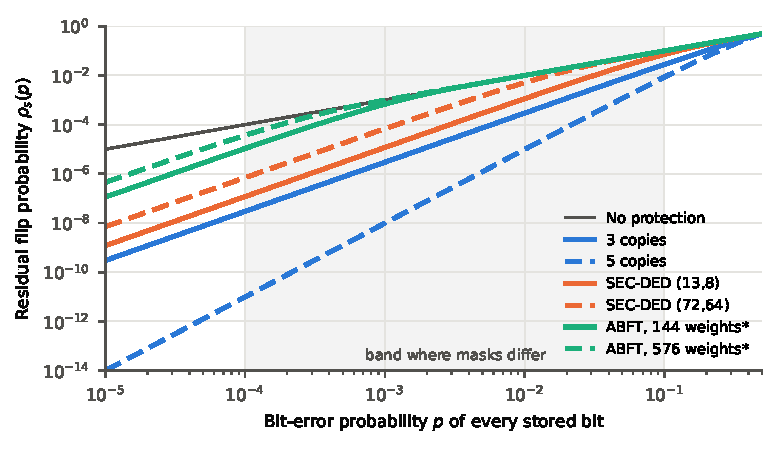
\includegraphics[width=.72\linewidth]{residual_curves}
\caption{Residual flip probability of a protected data bit against the bit-error probability of every stored bit, from Table~\ref{tab:mechanisms}. Copies keep a power law over the whole range. Codes and checksum correction leave it once a second error in the same word or channel becomes likely, near $p\approx1/n$ or $1/(8G)$, and then protect almost nothing. The shaded band is where the masks of this study differ. Curves are analytic; \Branch{R3a}{a bit-level simulation matches every one of them (Section~\ref{sec:mechanisms}).}{\TBD{simulation check outcome}.}}\label{fig:residual}
\Description{Log-log curves of residual error probability for no protection, three and five copies, two SEC-DED codes and two ABFT channel sizes.}
\end{figure}

\paragraph{Why stored weights, and why dense fault rates.} A stored weight is needed for the whole deployment and an activation only until it is consumed, so in the architectural-vulnerability view a weight bit is exposed for much longer~\cite{mukherjee2003avf,deutsch2024delayavf}. On the Eyeriss accelerator the projected failure rate of the filter memory exceeds that of the whole datapath by about three orders of magnitude, although which storage dominates depends on the architecture~\cite{li2017understanding,tyagi2023thales}. Proton tests of ECON-D, a radiation-hard ASIC of the CMS calorimeter upgrade~\cite{cummings2023econd}, combined with the planned luminosity of the High-Luminosity LHC~\cite{hllhc2017tdr}, imply that an unprotected register bit that is never rewritten reaches an upset probability of $10^{-3}$ within hours to days and $10^{-2}$ within days to weeks of beam, the band in which the masks of this study differ. Appendix~\ref{app:faultmotivation} gives the numbers and their limits; neither argument calibrates $p$. Because $p$ grows with the time since the last rewrite, scrubbing moves a deployment along these curves, which is one reason to design for a range of rates rather than for one.

\section{Why the Preferred Ranking Depends on the Fault Rate}\label{sec:theory}\label{sec:allocation}
\subsection{Protection value depends on what else fails}
Let $J_p(A)=\E_x\E_\xi[L_x(\theta+X)]$ be the expected loss of the faulty model under assignment $A$, where $x$ is an input, $L_x$ its loss, and $X$ the random displacement of the weights. For ideal suppression and an unprotected bit $b$, let $G$ be the random set of faults on the other unprotected bits. Because bit $b$ fails independently of $G$,
\begin{equation}\label{eq:protection-benefit}
J_p(A)-J_p(A\cup\{b\})=p\,\E_G\big[L(G\cup\{b\})-L(G)\big].
\end{equation}
This is the improvement potential of reliability theory, the failure probability times Birnbaum's importance~\cite{birnbaum1969importance,rausand2004system}. The expectation on the right is the damage of flipping $b$ in a network that already carries the faults $G$, and $G$ depends on $p$ and on the rest of the assignment. A ranking computed once ignores both. The rest of this section shows how they enter for a neural network, and when they matter.

\subsection{Mean and variance of the faulty weights}
Each weight moves by the sum of the jumps of its flipped bits, $X_w=\sum_{b:\,w(b)=w}\xi_b\Delta_b$ with $\xi_b\sim\mathrm{Bernoulli}(r_b)$ independent for unprotected and replicated bits. Its mean and variance are exact:
\begin{equation}\label{eq:moments}
\mu_w=\sum_{b:\,w(b)=w}r_b\,\Delta_b,\qquad V_w=\sum_{b:\,w(b)=w}r_b(1-r_b)\,\Delta_b^2 .
\end{equation}
Expanding the loss to second order around the average faulty weights $\theta+\mu$, the linear term vanishes in expectation and
\begin{equation}\label{eq:jhat}
J_p(A)\approx\hat J_p(A)=\underbrace{L(\theta+\mu)-L(\theta)}_{\text{loss at the average faulty weights}}+\underbrace{\tfrac12\textstyle\sum_w F_w V_w}_{\text{spread around them}},
\end{equation}
with $L=\E_xL_x$ and the curvature $F_w=\E_x[g_{x,w}^2]$, the mean squared gradient of weight $w$, standing in for the diagonal of the Hessian~\cite{lecun1989optimal,hassibi1992surgeon}. Only the diagonal is needed because the displacements of different weights are uncorrelated. The first term is evaluated exactly, by one forward pass of the model at $\theta+\mu$; only the spread around the average is approximated.

\subsection{One term per bit, one term per pair}
For ideal suppression, $r_b=p$ on the unprotected set $U$ and $0$ elsewhere. Writing $e_{x,b}=g_{x,w(b)}\Delta_b$ for the first-order effect of flipping $b$ on input $x$ and expanding Eq.~\eqref{eq:jhat} in $p$ (Appendix~\ref{app:theory}),
\begin{equation}\label{eq:p-expansion}
\hat J_p(A)=p\sum_{b\in U}\Big(\E_x e_{x,b}+\tfrac12\E_x e_{x,b}^2\Big)\;+\;\tfrac12p^2\!\!\sum_{\substack{b\ne b'\in U}}\!\!\E_x\big[e_{x,b}\,e_{x,b'}\big]\;+\;O(p^3).
\end{equation}
The first sum has one term per bit. While it dominates, the best mask protects the bits with the largest $\E_x e_{x,b}+\tfrac12\E_x e_{x,b}^2$, and a fixed ranking is optimal. The term keeps the \emph{sign} of the mean effect: a flip that lowers the loss on average is worth leaving unprotected, because a few such faults act like a small training step. The second sum has one term per pair of unprotected bits. It is large when many unprotected flips push the weights in the same direction, and no ranking can capture it, because the value of protecting one bit then depends on which others are protected. Fault rate decides which sum dominates: the per-bit sum grows like $p$ and the pairwise sum like $p^2$.

\subsection{The switch rate}
Compare a mask that leaves loss-lowering flips unprotected with one that leaves a balanced remainder. Their difference in Eq.~\eqref{eq:p-expansion} is approximately $D(p)=-a\,p+b\,p^2$ with $a,b>0$: the first mask gains $a\,p$ from the signed term and pays $b\,p^2$ for its one-sided remainder. The second mask becomes the better one above
\begin{equation}\label{eq:pstar}
p^*\approx\frac{a}{b}\approx\frac{2\,|g^\top v|}{v^\top H v},
\end{equation}
where $v$ is the summed jump of the one-sided remainder and $g$ the mean gradient. The remainder acts like a gradient step of size $p$ along $v$: it lowers the loss until the step is about twice the best step size along that direction, and raises it beyond. A model far from a minimum of its loss, with a large mean gradient, has a large $p^*$; a model at a minimum has $p^*\to0$, and the sign is never worth exploiting. In practice we do not use Eq.~\eqref{eq:pstar} but compute $\hat J_p$ of both masks on a grid of rates from calibration data, with the first term of Eq.~\eqref{eq:jhat} evaluated exactly, and locate the sign change of their difference. No fault is injected.

\subsection{What static rankings optimize}
Each static ranking of Table~\ref{tab:methods} is the exact optimum of one simplified piece of Eq.~\eqref{eq:p-expansion}, or close to one:
\begin{itemize}
\item The \emph{positive gradient}, $\E_x\max(0,e_{x,b})=\tfrac12(\E_x|e_{x,b}|+\E_x e_{x,b})$, is half the signed mean that drives the per-bit term plus half the absolute gradient. It is not the per-bit term itself, but it is the only static ranking that keeps the sign of the mean effect, so it should win at sparse rates and lose once the pairwise term matters.
\item The \emph{squared effect}, $\E_x e_{x,b}^2$, is the variance term alone.
\item The \emph{absolute gradient}, $\E_x|e_{x,b}|$, minimizes $\sum_{b\in U}\E_x|e_{x,b}|$, which bounds the per-input first-order damage when every unprotected flip happens to push the same way. Being sign-blind, it leaves a balanced remainder, so it should be close to the best choice at dense rates and never far behind at sparse ones.
\item \emph{Significance-first} and the \emph{numerical jump} rank by $|\Delta_b|$, the variance term with equal curvature for every weight, which is far from true in a trained network.
\item The \emph{global gradient}, $|\E_x e_{x,b}|$, keeps the size of the mean effect but drops its sign.
\end{itemize}
These readings are predictions about where each ranking does well. Section~\ref{sec:switch} tests the first of them directly.

\subsection{Calibration noise}
The signed mean $\E_x e_{x,b}$ is a sum of per-input terms that largely cancel, so it is small next to its own spread and needs many calibration inputs to estimate. The absolute and squared effects do not cancel. This is why masks that use the sign need hundreds of inputs while the absolute-gradient mask is settled at 64 (Appendix~\ref{app:calibration}). The method of Section~\ref{sec:method} shrinks every mean gradient toward zero by its standard error, so that where the sign is not resolved it falls back on magnitude.

\subsection{Imperfect protection, grouped failures and wrong repairs}\label{sec:theory-abft}
Equations~\eqref{eq:moments} and~\eqref{eq:jhat} hold for any per-bit rates $r_b=\rho_{A(b)}(p)$, so protection by copies enters by its residual curve. Codes and checksum correction add one more term, because the bits of one word or channel fail together: when a SEC-DED word holds two errors, both stay. The spread then gains $\tfrac12\sum_{b\ne b'}\mathrm{Cov}(\xi_b,\xi_{b'})\,\E_x[e_{x,b}e_{x,b'}]$ over pairs in the same group (Appendix~\ref{app:theory}). A checksum decoder can also make things worse. With two checksums $C_1=\sum_iq_i$ and $C_2=\sum_i i\,q_i$ over the codes of a channel, one faulty weight is located exactly, but two faulty weights produce a location $\sigma_2/\sigma_1$ that can point at a third, healthy weight, which is then changed. Which pairs of flips do so is fixed by the stored codes, so the rate of wrong repairs in a channel is $p^2$ times a count that can be computed once. On the pinned ResNet-8 \TBD{Stage 0 count: about 19\% of pairs of data-bit flips in different weights of a channel, and about 14\% of pairs of one data bit and one checksum bit, end in a wrong repair}. A real ABFT that checks computed outputs, rather than stored weights, has data-dependent locations and is not modelled.

\subsection{Where the approximation is weak}
Equation~\eqref{eq:jhat} is a second-order description of the spread. A sign or high-order flip is a large jump, and when several such jumps meet, the loss is no longer quadratic around the average weights. The expression also predicts loss, while designers care about accuracy or perplexity. Section~\ref{sec:method} therefore offers a Monte Carlo correction of exactly the part that is approximated, and Sections~\ref{sec:switch} and~\ref{sec:rateaware} judge every prediction by the task metric on independent fault fields.

\section{Rate-Aware Protection Assignment}\label{sec:method}
The cost $\hat J_p$ of Eq.~\eqref{eq:jhat} depends on $p$ and on the residual curves of the available mechanisms, so minimizing it gives an assignment that changes with the fault rate by construction. We minimize it for a given $p$ and storage budget $S$.

\paragraph{Ladders and moves.} The mechanisms available to a bit form a ladder of levels with equal storage steps: none and ideal suppression (one step of one bit), or none, three copies and five copies (two steps of two bits). Every move changes one bit by one level, so swapping $m$ step-ups for $m$ step-downs keeps the storage exactly at $S$. Codes and checksum correction protect whole words or channels and are compared as fixed, blanket mechanisms.

\paragraph{Value of a move.} The first-order change of $\hat J_p$ when bit $b$ moves from level $s$ to $s'$, per storage bit, is $-v_b$ with
\begin{equation}\label{eq:value}
v_b=\frac{(\rho_s-\rho_{s'})\big[\hat g_{w(b)}\Delta_b+\tfrac12(1-\rho_s-\rho_{s'})F_{w(b)}\Delta_b^2\big]}{\mathrm{cost}_{s'}-\mathrm{cost}_s}.
\end{equation}
The gradient $\hat g$ is taken at the average faulty weights $\theta+\mu$ of the current assignment, not at $\theta$. At small $p$, $\mu\approx0$ and $v_b$ is the signed per-bit term of Eq.~\eqref{eq:p-expansion}. At larger $p$ the gradient at $\theta+\mu$ reflects the overshoot of the current remainder, so bits whose flips would push further in the same direction gain value and bits whose flips push back lose it. The switch of Section~\ref{sec:theory} happens inside the search, without a threshold.

\paragraph{Search.} Starting from the better of two assignments, the absolute-gradient ranking and the ranking by $v_b$ at $\mu=0$, each round computes $\mu$ and $\hat g$ with one forward and one backward pass over the calibration inputs, swaps the $m$ best step-ups for the $m$ cheapest step-downs, and keeps the swap if $\hat J_p$ falls; otherwise $m$ is halved. The search stops when $m<16$ or after 40 rounds. Every round records the cost and its parts, the storage used, the number of bits at each level and the distribution of $v_b$ over all moves and over the chosen ones, so the course of the optimization can be inspected (Appendix~\ref{app:runr}).

\paragraph{Calibration noise.} Each mean gradient is shrunk by its standard error over the calibration inputs, $\tilde g_w=\bar g_w\max(0,1-\mathrm{se}_w^2/\bar g_w^2)$, so the signed term vanishes where its sign is not resolved.

\paragraph{Monte Carlo correction.} The part of $\hat J_p$ that is approximated is the spread around the average weights. With $K$ fault fields drawn once and shared by every candidate assignment, the correction $\hat C=\frac1K\sum_k[L(\theta+X_k)-L(\theta+\mu)]-\tfrac12\sum_wF_wV_w$ replaces that approximation by a sample, and the mean gradient over the $K$ faulted models replaces $\hat g$. The correction samples only what the expression misses, and the shared fields make differences between candidates far less noisy than the objective itself. \TBD{$K$ and the refresh interval, from the Stage 0 rule.}

\paragraph{Annealing.} As an optional variant, swaps are sampled with probability proportional to $\exp(v_b/T)$ and a worse assignment is accepted with probability $\exp(-\Delta J/T)$, with $T$ set by the first rejected step and lowered by 10\% per round. It is kept only if it improves on plain descent (rule R2c).

\paragraph{Outputs.} For a rate or a range of rates and a set of available mechanisms, the method returns the assignment, the predicted loss of every candidate against $p$, the predicted switch rates between the simple rankings, the loss of each assignment when the rate is misjudged, and a map of how many bits of each layer and bit position receive each mechanism. A designer who knows the operating regime, for example from the scrubbing interval, can read off whether a simple ranking is enough there.

\paragraph{Cost.} On ResNet-8 one analytic assignment takes \TBD{seconds, from Stage 0} on two CPU threads, and the corrected one \TBD{seconds}. The per-input gradients are those already needed by the absolute-gradient ranking.

\section{Experimental Methodology}\label{sec:experiments}
\subsection{Static rankings}\label{sec:susceptibility}\label{sec:estimators}
Each static ranking orders the eligible bits, and protecting the first $B$ gives an exact-budget mask (Table~\ref{tab:methods}). With $e_{x,b}=g_{x,w(b)}\Delta_b$, the three gradient rankings aggregate the same per-example effects differently; Section~\ref{sec:theory} relates each to a piece of the expected loss. For FKeras~\cite{weng2024fkeras} we use the published projection $H'=\sum_{k=1}^{r}\lambda_k(v_k^\top\theta)v_k$ with $r=2$ signed largest-magnitude eigenpairs of a continuous loss Hessian, and order bits by significance tier and then by $|H'_i|$. The gradient companions use straight-through requantization and the Hessian companion omits activation rounding; neither differentiates the integer program (Appendix~\ref{app:implementation}). At 12.5\% and 25\% coverage MSB-first and FKeras protect the same complete tiers and are counted as one decision (Appendix~\ref{app:repeated}).

\begin{table}[t]
\caption{Static rankings. Larger scores rank first; $\E_x$ averages calibration inputs and $j$ is the bit position. Remaining ties follow the stored tensor, word and bit order.}\label{tab:methods}
\centering\small
\begin{tabularx}{\linewidth}{l l X}\toprule
Ranking & Score or ordering & Needs\\\midrule
Random & Seeded permutation & Nothing\\
MSB-first & Descending $j$ & Bit positions\\
Numerical jump & $|\Delta_b|$ & Stored codes and scales\\
Global gradient & $|\E_x e_b(x)|$ & Labelled calibration set, one mean gradient\\
Absolute gradient & $\E_x|e_b(x)|$ & Labelled calibration set, per-example gradients\\
Positive gradient & $\E_x\max(0,e_b(x))$ & Same as absolute gradient\\
FKeras & Descending $j$, then $|H'_i|$ & Calibration set, two Hessian eigenpairs\\\bottomrule
\end{tabularx}
\Description{Seven ranking methods differ in their scores, aggregation and required information.}
\end{table}

\subsection{Models and operating grid}
Table~\ref{tab:models} lists the six frozen studies. The three MLPerf Tiny models are the reference INT8 TFLite files with their reference preprocessing~\cite{banbury2021mlperf,mlcommons2026tiny}: ResNet-8 on CIFAR-10, DS-CNN on Speech Commands~\cite{warden2018speechcommands}, and the ToyCar autoencoder on ToyADMOS~\cite{koizumi2019toyadmos}, run on the TensorFlow Lite 2.14.1 reference kernels. DistilBERT on SST-2~\cite{sanh2019distilbert,socher2013sentiment}, Pythia-160M~\cite{biderman2023pythia} and Qwen3-0.6B~\cite{yang2025qwen3} are W8A8 executables derived from the public checkpoints, with per-channel symmetric INT8 weight codes, per-token activation quantization and exact INT32 accumulation; the language models are scored on WikiText-2~\cite{merity2017pointer}. Appendix~\ref{app:implementation} gives checkpoint identities and quantization rules.

\begin{table}[t]
\caption{Frozen models, eligible populations and evaluation cohorts. $Np$ is the expected number of proposed faults per field at the lowest BER. Clean quality is measured on the listed cohort.}\label{tab:models}
\centering\small
\begin{tabular}{l r r l r l}\toprule
Model & Eligible bits $N$ & $Np$ at $10^{-5}$ & Cohort & Fields/BER & Clean quality\\\midrule
ResNet-8 & 618,880 & 6.2 & 1,000 images & 32 & 88.0\% accuracy\\
DS-CNN & 176,128 & 1.8 & 1,000 clips & 32 & 90.1\% accuracy\\
ToyCar & 2,113,536 & 21 & 64 files & 32 & 0.869 file AUC\\
DistilBERT & 344,469,504 & 3,445 & 512 sentences & 24 & 91.4\% accuracy\\
Pythia-160M & 988,545,024 & 9,885 & 4,096 tokens & 24 & 3.530 nats/token\\
Qwen3-0.6B & 4,767,875,072 & 47,679 & 4,096 tokens & 24 & 2.829 nats/token\\\bottomrule
\end{tabular}
\Description{Six models with eligible bit counts, expected fault counts, cohorts, fields per BER and clean task quality.}
\end{table}

Every study evaluates 6.25\%, 12.5\%, 18.75\% and 25\% protection, with unprotected and fully protected controls, at BERs of $10^{-5}$, $10^{-4}$, $3\!\times\!10^{-4}$, $10^{-3}$, $3\!\times\!10^{-3}$, $10^{-2}$, $3\!\times\!10^{-2}$ and $10^{-1}$; ToyCar omits $3\!\times\!10^{-4}$, $3\!\times\!10^{-2}$ and $10^{-1}$. A (BER, budget) pair is a \emph{cell}. All six non-Hessian rankings are measured in every cell, FKeras on the three TFLite models only, for 1,254 method-cell conditions and 35,136 saved policy-field outcomes. Rankings use 64 calibration inputs for ResNet-8, DS-CNN and DistilBERT, 16 normal training files for ToyCar, and 8,184 validation targets for each language model. Evaluation inputs are disjoint from calibration inputs, but several cohorts were used in earlier exploratory runs.

\paragraph{Task metrics.} Classifiers are judged by accuracy. TFLite cross-entropy, computed from the 8-bit softmax output, is dominated by zero-probability outputs and is not used for conclusions. ToyCar is judged by ROC-AUC over 64 files, with one fault state per file. Language models are judged by mean token negative log-likelihood (NLL), capped at 30 nats per token, which is also the penalty for a nonfinite output; none occurred. Appendix~\ref{app:implementation} gives the exact definitions.

\subsection{Usefulness criterion}
Comparisons between masks only matter where at least one of them leaves a usable model. We therefore fixed the following criterion before computing any regret, although after the fault data had been collected and two slices of the grid had been plotted. A method is \emph{useful} in a cell if its mean accuracy or file AUC is within 0.05 of the clean value, or, for a language model, if its mean NLL is within 0.5 nats per token of clean (a perplexity ratio of at most 1.65). A cell is \emph{decision-useful} if at least one measured ranking is useful there. Margins of 0.01/0.1 and 0.10/1.0 are used as sensitivity checks.

\subsection{Statistics}
In the main grid the independent unit is the fault field. All contrasts between masks are paired on the field, intervals are two-sided 95\% Student-$t$ intervals on the paired differences, and tests are paired sign-flip tests with 20,000 random sign assignments. Holm correction is applied within each model over all contrasts between the absolute-gradient mask and every other mask on the whole grid (120 to 192 contrasts); statements about other pairs use the family of all pairwise contrasts. A difference is \emph{resolved} when its Holm-adjusted $p$ is below 0.05, and identical masks are counted once. The \emph{regret} of a ranking in a cell is its paired mean risk minus that of the best measured ranking in the same cell; because the best ranking is chosen on the same fields, regrets are biased slightly upward. These intervals describe fault randomness only and condition on one checkpoint, one cohort and one mask per deterministic ranking and budget.

\subsection{Repeated evaluations of the static rankings}\label{sec:repeated}\label{sec:confirm}
The two TFLite classifiers were evaluated again in replications that each draw their own 64 calibration inputs, rebuild every mask, evaluate their own input window and propose new fault fields: nine ResNet-8 and eleven DS-CNN replications, with an analysis plan and decision rule fixed before the runs. Eight further ResNet-8 checkpoints were trained with the reference recipe: two pruned copies (50\% and 70\% of each layer's kernel weights), one trained for 100 instead of 500 epochs, and five retrained from scratch with different seeds (86.6\% to 87.2\% INT8 test accuracy). The gradient masks of all nine checkpoints were also rebuilt from 128 to 1,024 calibration inputs and replayed on the saved fault fields. Appendices~\ref{app:repeated}, \ref{app:calibration} and~\ref{app:static} give the designs and results.

\subsection{Confirmatory tests of the theory and the method}\label{sec:runr}
Every prediction and decision rule below was fixed in a written plan before the fault fields were drawn (Appendix~\ref{app:runr}). The tests use the nine ResNet-8 checkpoints, the replications and input windows of the repeated evaluations, and fresh fault fields whose random numbers are nested across rates and shared by every mask.
\begin{itemize}
\item \textbf{Stage 1, the switch.} Positive- and absolute-gradient masks from 1,024 calibration inputs at eight budgets from 1\% to 50\%, at twelve rates from $3\times10^{-4}$ to $3\times10^{-2}$, eight fields per replication. The predicted switch $p^*$ of every checkpoint and budget was computed from held-out training images and frozen by file hash. Rules: no resolved usable cell outside a factor 1.25 of $p^*$ has the wrong sign (R1a); at least 80\% of all such cells have the right sign (R1b); the measured switch is within a factor 1.5 of $p^*$, with a 95\% interval over the nine checkpoints (R1c).
\item \textbf{Stage 2, the rate-aware assignment.} Six static masks (the paper's absolute gradient from 64 inputs; absolute, positive and squared effect from 1,024; FKeras; significance-first) and two versions of the assignment (analytic, and with the Monte Carlo correction), each built for the rate at which it is tested, at four budgets from 6.25\% to 25\% and eight rates from $10^{-4}$ to $3\times10^{-2}$. On two checkpoints every built-for rate is also tested at every rate. Rule R2a: no other mask is ahead of the analytic assignment by half a point or more in a usable cell after Holm correction; R2b: the absolute and the positive gradient each fail the same test on at least seven of nine checkpoints; R2c: the correction is kept only if it is resolved ahead of the analytic version on at least three checkpoints and behind on none.
\item \textbf{Stage 3, mechanisms.} Each residual curve of Table~\ref{tab:mechanisms} against a bit-level simulation of its mechanism (R3a), and accuracy at equal extra storage of ranked triplication, rate-aware triplication, a rate-aware choice between three and five copies, SEC-DED codes and ABFT (R3b).
\item \textbf{Stage 4, a second model.} The DS-CNN with six replications, each with its own 1,024 calibration clips and its own window of 800 test clips, at budgets of 12.5\% to 37.5\%, where its predicted switch lies inside the usable range. Stage 1 and the analytic assignment of Stage 2 are repeated against five static masks (absolute and positive gradient from 1,024 clips, the paper's absolute gradient from 64, FKeras and significance-first). \TBD{Stage 4 outcome.}
\end{itemize}

\subsection{Compute}\label{sec:cost}
All experiments ran on one server with two Intel Xeon Gold 6248 processors (40 cores, 80 hardware threads) and 472\,GiB of memory, without a GPU. Every faulty-model outcome comes from the TFLite reference kernels on one thread, and jobs ran as up to 76 single-threaded processes, so two jobs usually shared one core. Stage 1 took 345 CPU hours for 110,592 evaluations (12.2\,s each on a shared core, 6.2\,s alone) and about five hours of wall time. \TBD{Table of CPU hours per stage, per mask and per evaluation, from the run ledger, once Stages 2 and 4 end.}

\section{Results}\label{sec:results}
\subsection{Static rankings: the choice matters where the model is still useful}\label{sec:static}
Figure~\ref{fig:ber} shows task quality against BER at 12.5\% protection. At low BER all masks are indistinguishable from clean operation, and at the highest BERs every mask fails. In between lies a band, one to two decades wide, where the model is useful under some masks and not under others; that band is where protection decisions have consequences. For ResNet-8 at $p=3\times10^{-3}$, accuracy is 36.8\% unprotected, 70.3\% with MSB-first, 80.9\% with the global gradient and 83.0\% with the absolute gradient, against 88.0\% clean; the paired gain of absolute gradient over MSB-first is 12.7 points (95\% interval 8.4 to 16.9). For Qwen3-0.6B at $p=3\times10^{-3}$ the NLL increase is 7.60 nats per token unprotected, 0.88 with MSB-first and 0.27 with either gradient ranking.

\begin{figure}[tbp]
\centering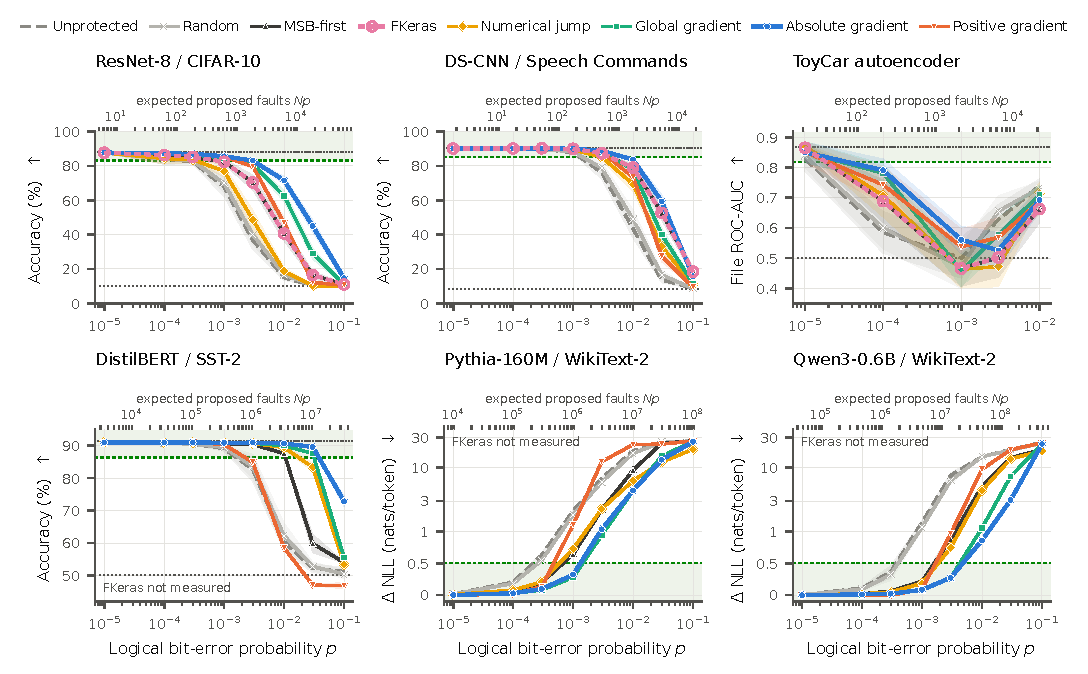
\includegraphics[width=\linewidth]{tecs_task_quality_ber_125}
\caption{Task quality versus logical BER at 12.5\% protection, with the expected number of proposed faults on the top axis. Bands are 95\% intervals of the field mean. The shaded region is the usefulness margin; dotted lines mark clean quality and chance. FKeras (open circles) was measured on the three TFLite models only; at this complete-tier budget it selects the same mask as MSB-first. Language-model panels use a symmetric-log axis.}\label{fig:ber}
\Description{Six panels of accuracy, AUC or NLL against bit-error probability for seven protection policies.}
\end{figure}

\begin{table}[t]
\caption{Highest measured BER, in units of $10^{-4}$, at which each ranking keeps mean task quality within the usefulness margin, at 12.5\% / 25\% protection. Unprotected has no budget. FKeras equals MSB-first at these two budgets.}\label{tab:useful}
\centering\small
\begin{tabular}{l r r r r r}\toprule
Ranking & ResNet-8 & DS-CNN & DistilBERT & Pythia & Qwen\\\midrule
Unprotected & 1 & 10 & 10 & 1 & 3\\
Random & 1 / 3 & 10 / 10 & 10 / 10 & 1 / 3 & 3 / 3\\
MSB-first & 3 / 10 & 30 / 100 & 100 / 100 & 3 / 10 & 10 / 30\\
Numerical jump & 3 / 3 & 10 / 30 & 100 / 300 & 3 / 10 & 10 / 30\\
Global gradient & 10 / 30 & 30 / 100 & 300 / 300 & 10 / 30 & 30 / 100\\
Absolute gradient & 30 / 30 & 30 / 100 & 300 / 1000 & 10 / 10 & 30 / 100\\
Positive gradient & 10 / 30 & 30 / 30 & 10 / 30 & 3 / 3 & 10 / 30\\\bottomrule
\end{tabular}
\Description{Highest useful bit-error probability for seven policies on five models at two budgets.}
\end{table}

Table~\ref{tab:useful} condenses the grid into the highest measured BER at which each ranking keeps the model useful. At 12.5\% protection the absolute-gradient mask extends the useful range over MSB-first by a factor of ten on ResNet-8 and three on DistilBERT, Pythia and Qwen, and over the unprotected model by three to thirty. These factors are resolved only to the half-decade grid and depend on the input window: on nine further ResNet-8 windows (Section~\ref{sec:default}) they are three and ten, while the accuracy losses at $3\times10^{-3}$ for absolute gradient, MSB-first and no protection (3.0, 16.1 and 44.5 points) agree with the original window (5.0, 17.7 and 51.2). ToyCar cannot inform the choice: its only decision-useful cells are the four at $p=10^{-5}$, where the unprotected model is itself useful (Appendix~\ref{app:evidence}).


Appendix~\ref{app:static} gives the detailed static-ranking results. With masks from 64 calibration inputs, the absolute-gradient mask keeps its largest regret below 0.7 accuracy points across new calibration draws, input windows, pruned checkpoints and retrained copies of ResNet-8, and no search-based or literature-derived allocator beats it by a point where the model is usable (Appendix~\ref{app:search}). Significance-first protection loses 9 to 34 points to it on every ResNet-8 checkpoint at $p=3\times10^{-3}$. The positive-gradient mask, which keeps the sign of a flip's effect, behaves as Section~\ref{sec:theory} predicts: on the language models it is best at the lowest rates and worst at moderate ones, on DistilBERT and Pythia it is worse than no protection in several cells, and on the under-trained ResNet-8 it lifts accuracy above the clean model at $p=10^{-3}$ and loses 22.6 points at $10^{-2}$. With 1,024 calibration inputs the same reversal appears on all nine ResNet-8 checkpoints: the positive-gradient mask is ahead in every usable cell at $10^{-3}$ and behind in every usable cell at $10^{-2}$, with resolved wins in both directions on five checkpoints (Appendix~\ref{app:calibration}). The rest of this section tests whether the theory predicts these switches and whether an assignment built from it avoids them.

\subsection{Predicting where the preferred ranking switches}\label{sec:switch}
\begin{figure}[t]
\centering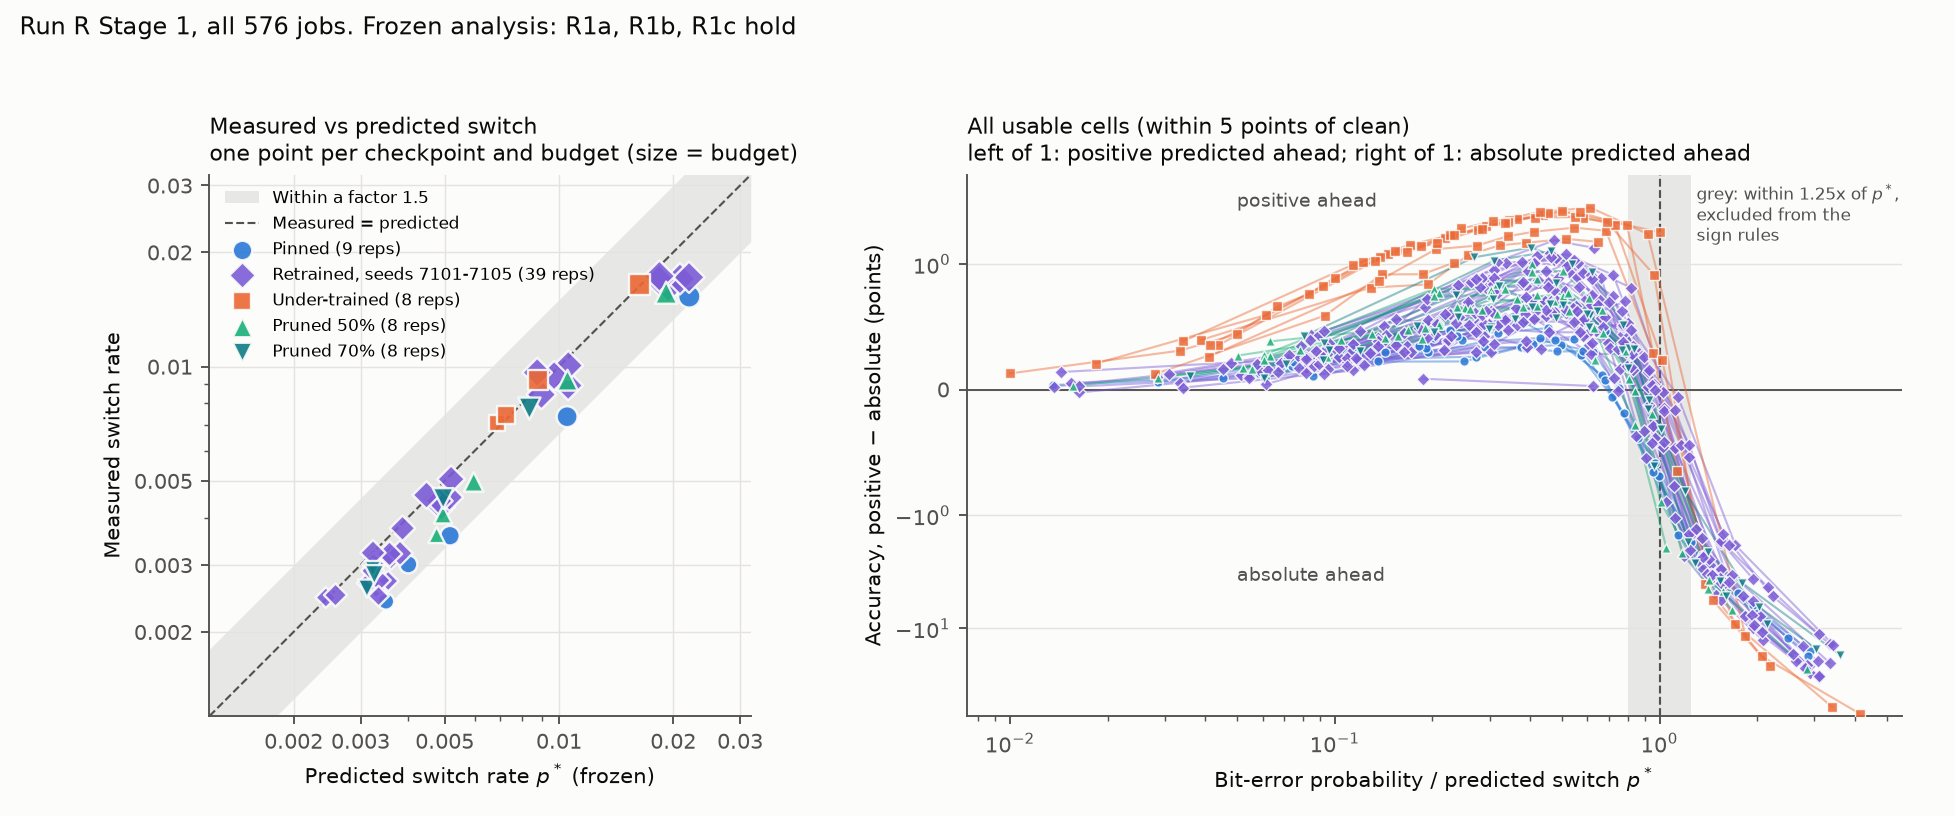
\includegraphics[width=\textwidth]{figures/stage1_switch.png}
\caption{Predicted and measured switch between the positive- and absolute-gradient masks on nine ResNet-8 checkpoints. Left: measured against predicted switch rate, one point per checkpoint and budget, with the factor-1.5 band fixed in advance. Right: accuracy of the positive minus the absolute mask in every usable cell, against the bit-error probability divided by its predicted switch; all curves cross zero near 1. The predicted switch is computed from 512 held-out training images without fault injection and was frozen before the fault fields were drawn.}\label{fig:switch}
\Description{Measured accuracy difference between two gradient masks against bit-error probability, with the predicted switch rate.}
\end{figure}
Figure~\ref{fig:switch} compares the predicted switch with the measurement on fresh fault fields. \Branch{R1}{The sign of the measured difference agrees with the prediction in 515 of the 519 usable cells away from the switch, and in all 404 of them that are resolved after Holm correction; the four exceptions are below 0.2 points. The measured switch is 0.88 times the predicted one (95\% interval over the nine checkpoints 0.80 to 0.96), within the factor of 1.5 fixed in advance. It moves with the budget as predicted, from about $2.6\times10^{-3}$ at 6.25\% to about $1.5\times10^{-2}$ at 50\% (geometric means over checkpoints), and it is highest on the under-trained checkpoint, the one farthest from a minimum ($9.5\times10^{-3}$ against $4.8$ to $5.8\times10^{-3}$ for the well-trained ones). Below 6.25\% the network loses more than 5 points before the masks swap order, so no switch is measured there.}{\TBD{Which of R1a, R1b and R1c failed, and by how much.} The prediction \TBD{e.g., gets the sign right but places the switch \ldots}.} The formula places the switch about 12\% late on average (geometric mean of measured over predicted 0.88), most on the pinned checkpoint (0.71) and least on the under-trained one (1.03). A designer who simply follows the predicted switch, positive below $p^*$ and absolute above, loses 0.01 accuracy points on average against the better of the two masks, at most 0.19 points away from the switch and at most 1.9 points next to it.

\subsection{Rate-aware assignment against static rankings}\label{sec:rateaware}
\begin{figure}[t]
\centering\TBDfig{5cm}{Stage 2. Left: for each mask, the gap to the best mask in each usable cell against $p$ (nine checkpoints, four budgets); the headline is the largest gap. Right: misjudged rate, gap of a mask built for $p_a$ and tested at $p_b$ (8$\times$8, pinned and under-trained).}
\caption{\TBD{Stage 2 caption.}}\label{fig:rateaware}
\Description{Gap to the best mask against bit-error probability for static rankings and the rate-aware assignment.}
\end{figure}
\Branch{R2}{The analytic rate-aware assignment is never resolved behind another mask by half a point or more in a usable cell on any of the nine checkpoints; its largest gap is \TBD{}. The absolute-gradient mask falls behind by \TBD{} on \TBD{n} checkpoints, mostly at sparse rates, and the positive-gradient mask by \TBD{} on \TBD{n}, at dense rates.}{\TBD{Stage 2 outcome: where the assignment fell behind and by how much.}} \Branch{R2c}{The Monte Carlo correction \TBD{improves on the analytic version where several large jumps meet, at \ldots}.}{The Monte Carlo correction and annealing did not improve on the analytic version and are not part of the method.} When the rate is misjudged, \TBD{cost of building for $p_a$ and running at $p_b$; e.g., building for a rate below the true one costs \ldots}.

\subsection{Protection mechanisms at equal storage}\label{sec:mechanisms}\label{sec:correction}
A ranking chooses which bits a mechanism covers, not the mechanism. To see whether that choice matters against mechanisms that cover every bit, we compared on ResNet-8, at equal extra storage, triple modular redundancy (TMR) of the bits selected by the absolute-gradient mask with three blanket schemes: a SEC-DED Hamming code over words of 64, 32, 16 or 8 weight bits, which repairs one flipped bit per word; ABFT checksum correction, which stores two weighted checksums per output channel and repairs one faulty weight per channel, applied to the stored weights, which favours it; and TMR of every sign bit, which corresponds to FORTUNE-style protection~\cite{nazari2024fortune}. Every stored bit flips with probability $p$, including copies and check bits, so a triplicated bit is wrong after voting with probability $3p^2-2p^3$; miscorrection of three or more errors is ignored, which favours the codes. The study uses the TFLite executable, test images 1000 to 1999, the absolute-gradient mask built for that window in the repeated evaluation, and eight fault draws per BER.

\begin{figure}[tbp]
\centering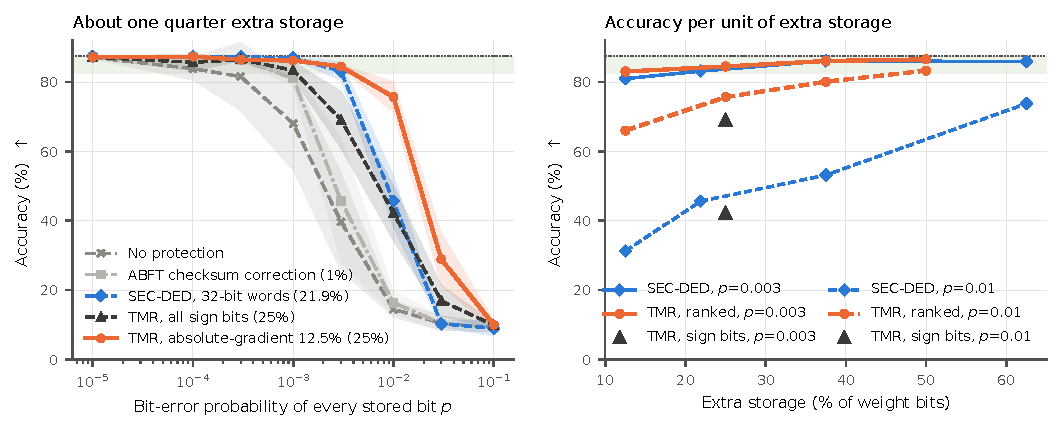
\includegraphics[width=\linewidth]{tecs_correction_mechanisms}
\caption{ResNet-8, protection mechanisms at equal extra storage. Every stored bit, including copies and check bits, flips with probability $p$. Bands are 95\% intervals over eight fault draws; the shaded region is the usefulness margin. Left: schemes costing about a quarter of the weight storage. Right: accuracy against extra storage at $p=3\times10^{-3}$ (solid) and $10^{-2}$ (dashed). ABFT checksum correction stores two checksums per output channel ($\approx$1\%).}\label{fig:correction}
\Description{Accuracy against bit-error probability and against extra storage for TMR of ranked bits, SEC-DED codes, ABFT checksum correction and TMR of sign bits.}
\end{figure}

The outcome depends on the fault rate (Fig.~\ref{fig:correction}). Up to $p=10^{-3}$ the codes are slightly better, by 0.7 to 1.4 accuracy points; near $3\times10^{-3}$ the two are equivalent; from $10^{-2}$ on, triplicating ranked bits is far better. At $p=10^{-2}$ and 12.5\% extra storage it keeps 66.0\% accuracy against 31.3\% for SEC-DED over 64 bits, a paired difference of 34.7 points (interval 25.7 to 43.8); at 25\% it keeps 75.7\% against 45.6\% for SEC-DED over 32 bits (21.9\% storage) and 42.3\% for TMR of all sign bits. Against sign-bit TMR of equal cost the ranked mask is better at every BER from $10^{-3}$ on, by 15.4 points (7.1 to 23.6) at $3\times10^{-3}$. ABFT checksum correction recovers almost nothing above $10^{-3}$, because almost every output channel then holds two or more faulty weights. Codes fail when two errors land in one word, which becomes likely at dense fault rates, while TMR of a bit fails only when two of its own three copies flip. By the usefulness criterion the gain is smaller: at 25\% and 37.5\% storage both ranked TMR and the code stop at $3\times10^{-3}$. The comparison counts storage only; voters, encoders, decoders, interleaving and scrubbing are not modelled, and it covers one checkpoint and one input window.


\Branch{R3a}{A bit-level simulation of each mechanism matches its residual curve in Table~\ref{tab:mechanisms} at every rate \TBD{}, including the wrong-repair rate of the checksum decoder.}{\TBD{which curves departed from simulation}.} The curves explain the ordering above: codes keep a $p^2$ law only while a second error in a word is unlikely, near $p<1/n$, and checksum correction over channels of hundreds of weights leaves it already near $p\approx10^{-4}$ (Fig.~\ref{fig:residual}). \Branch{R3b}{Letting the rate-aware assignment choose between three and five copies per bit improves on ranked triplication by \TBD{} at equal storage.}{Choosing between three and five copies per bit did not improve on ranked triplication \TBD{}.}

\section{Discussion and Limits}\label{sec:discussion}
\paragraph{What a designer can take from this.} First, a fixed ranking is a bet on the fault rate. The per-bit term of Eq.~\eqref{eq:p-expansion} rewards rankings that keep the sign of a flip's effect when faults are sparse; the pairwise term rewards balanced, sign-blind rankings when they are dense; and the rate at which one takes over can be computed before any fault is injected. \Branch{R1}{On ResNet-8 that computation located the switch within a factor of 1.5 of where it was measured on every checkpoint, about 12\% late on average.}{\TBD{How far the computed switch can be trusted, given Stage 1.}} Second, when the rate is not known, the absolute gradient is the safe static choice: it never fell far behind in the static evaluation, while the positive gradient lost up to 18 points where faults were dense and significance-first protection 9 to 34 points at a moderate rate. Third, \Branch{R2}{when the rate is known or bounded, the rate-aware assignment removes the bet: on ResNet-8 it was never more than half a point behind the best tested mask \TBD{}.}{\TBD{what the rate-aware assignment does and does not buy, from Stage 2}.} Fourth, protection should be judged by its residual error curve, not by its name. Codes and checksum correction keep a quadratic residual only while a second error per word or channel is unlikely; beyond that they protect almost nothing, while copies keep their power law (Fig.~\ref{fig:residual}). At dense fault rates, triplicating ranked bits beat SEC-DED codes and checksum correction of equal storage by 30 points or more on ResNet-8.

\paragraph{Why not search for the mask by fault injection?} A Monte Carlo search estimates the same expected loss by sampling and needs many fault fields to resolve differences of a fraction of a point; on the pinned ResNet-8 such a search and a relaxed per-bit optimizer did not beat the absolute-gradient mask where the model is usable, and the relaxed optimizers lost 4 to 12 points there (Appendix~\ref{app:search}). The expression of Section~\ref{sec:theory} computes the expectation in closed form, to second order around the average faulty weights, and samples only the part it approximates. \Branch{R2c}{The sampled correction helped where \TBD{}.}{The sampled correction did not help on ResNet-8.}

\paragraph{Limits.} The theory is a second-order description around the average faulty weights and predicts loss, not accuracy. The confirmatory tests cover nine ResNet-8 checkpoints, and one further model, the DS-CNN, is checked with a smaller design (\TBD{Stage 4 outcome}); the other four models enter through the static evaluation only. The prediction places the switch about 12\% late on ResNet-8, and below 6.25\% protection the switch falls where the model is no longer usable, so the prediction is tested only from 6.25\% up. Each model except ResNet-8 has one trained checkpoint, several input cohorts had been used before, and the derivation was written after the reversal of Appendix~\ref{app:calibration} had been observed, although every prediction tested in Section~\ref{sec:switch} was fixed before its fault fields were drawn. The residual curves assume independent faults, fault-free voters and decoders, and no miscorrection of three or more errors; the checksum decoder is applied to stored weights, which favours it, and an ABFT that checks computed outputs is not modelled. Counting storage bits ignores the area, power and latency of voters, decoders and their placement. Biases, scales, embeddings and normalization parameters are never faulted, and activation, datapath and control faults are outside the fault model. Logical $p$ is a model parameter, not a radiation rate, and the band in which masks differ, about $10^{-4}$ to $10^{-1}$, is a regime of dense memory errors that scrubbing would shorten~\cite{biswas2005avf}.

\section{Conclusion}\label{sec:conclusion}
Which stored bits are worth protecting depends on how many of them fail. The expected loss of a faulty model splits into a term per bit, which grows like the bit-error probability and favours protecting the flips that raise the loss on average, and a term per pair of bits, which grows like its square and favours leaving a balanced remainder; a fixed ranking is optimal only while the first dominates. \Branch{R1}{The rate at which the preferred ranking switches can be computed from calibration data, and on nine ResNet-8 checkpoints it agreed with the measurement within a factor of 1.5, about 12\% late on average.}{\TBD{Stage 1 outcome in one sentence}.} Because protection mechanisms only lower the probability of an error, the same expression takes the residual error curve of each one, \Branch{R2}{and an assignment that minimizes it for the given rate was never more than half a point behind the best tested mask on ResNet-8 \TBD{}.}{\TBD{Stage 2 outcome in one sentence}.} Across six frozen INT8 models, significance-first protection tolerates a fraction of the fault rate that gradient-based masks tolerate, and at dense fault rates triplicating well-chosen bits outperforms blanket codes and checksum correction of equal storage. All results assume logical faults with idealized voters and decoders.

\begin{acks}
AI-assisted tools supported software development, evidence organization, statistical re-analysis, figure preparation and drafting. The scientific claims in this manuscript are linked to the archived measurements and derivations identified in the accompanying evidence manifest. Responsibility for the submitted work rests with the authors.
\end{acks}
\bibliographystyle{ACM-Reference-Format}
\bibliography{references}
\appendix
\section{Derivations}\label{app:theory}
\paragraph{Exact moments.} In two's complement the change of a word caused by any set of flipped bits is the sum of the single-bit jumps, so $X_w=\sum_{b:\,w(b)=w}\xi_b\Delta_b$ holds exactly. With independent $\xi_b\sim\mathrm{Bernoulli}(r_b)$, $\E X_w=\sum r_b\Delta_b$ and $\mathrm{Var}X_w=\sum r_b(1-r_b)\Delta_b^2$, and displacements of different weights are independent.

\paragraph{Second order around the average weights.} Write $X=\mu+\varepsilon$ with $\E\varepsilon=0$. Then $L(\theta+X)=L(\theta+\mu)+\nabla L(\theta+\mu)^\top\varepsilon+\tfrac12\varepsilon^\top H(\theta+\mu)\varepsilon+O(\|\varepsilon\|^3)$, and taking expectations removes the linear term, leaving $\E L(\theta+X)\approx L(\theta+\mu)+\tfrac12\sum_w H_{ww}(\theta+\mu)\,V_w$, because $\varepsilon$ has a diagonal covariance. We use the Fisher diagonal at $\theta$, $F_w=\E_x g_{x,w}^2$, for $H_{ww}$.

\paragraph{Expansion in $p$.} For ideal suppression, $\mu=p\,v$ with $v=\sum_{b\in U}\Delta_b$ (as a vector over weights). Expanding the first term, $L(\theta+\mu)-L(\theta)=p\,g^\top v+\tfrac12p^2v^\top Hv+O(p^3)$, and with the Fisher approximation $H\approx\E_x g_xg_x^\top$, $v^\top Hv=\sum_{b,b'\in U}\E_x e_{x,b}e_{x,b'}$. The second term is $\tfrac12p(1-p)\sum_{b\in U}\E_xe_{x,b}^2$. Adding the two, the $p^2$ diagonal terms cancel, which gives Eq.~\eqref{eq:p-expansion}: a per-bit term in $p$ and a sum over distinct pairs in $p^2$.

\paragraph{Grouped failures.} For a SEC-DED word that leaves double errors as they are, two data bits of the word are both wrong after decoding exactly when both flipped, so $\mathrm{Cov}(\xi_b,\xi_{b'})=p^2-r_br_{b'}$ for $b\ne b'$ in the word. For one-weight checksum repair, two bits in different weights of a channel are both wrong when both flipped, $p^2$, and two bits of the same weight when both flipped and another weight of the channel is faulty. The extra spread is $\tfrac12\sum_{b\ne b'}\mathrm{Cov}(\xi_b,\xi_{b'})\E_x[e_{x,b}e_{x,b'}]$ over pairs in the same group, computed from per-input gradients summed per group.

\paragraph{Wrong repairs.} With integer errors $\delta_i$ in a channel and errors $\epsilon_1,\epsilon_2$ in the two checksum words, the decoder sees $\sigma_1=\sum_i\delta_i-\epsilon_1$ and $\sigma_2=\sum_ii\,\delta_i-\epsilon_2$. It does nothing if $\sigma_1=0$, subtracts $\sigma_1$ from weight $\ell=\sigma_2/\sigma_1$ if $\ell$ is an integer in $1,\dots,G$, and otherwise leaves the channel. One faulty weight is repaired exactly and one faulty checksum word alone changes nothing. For two faults, the outcome is fixed by the stored codes and the positions of the two flips, so all pairs can be enumerated once per channel; a wrong repair adds $-\sigma_1$ to weight $\ell$, which enters $\mu$ and $V$ with weight $p^2$.

\section{Confirmatory Tests: Design and Records}\label{app:runr}
\paragraph{Plan and records.} The tests of Sections~\ref{sec:switch} and~\ref{sec:rateaware} follow a written plan whose estimands, cohorts, rates, seeds, statistics and decision rules were fixed before the corresponding fault fields were drawn. Changes made before any outcome are recorded as amendments: the wider set of eight Stage~1 budgets, the removal of annealing, three details of the analysis that the plan had left open (a difference of exactly zero counts against the prediction; a checkpoint and budget whose difference never changes sign has no measured switch and is left out of rule R1c; clean accuracy is the mean over replications), and the constants of Stage~2. Two descriptive looks at partial Stage~1 data were taken; nothing was changed after them, except the size of a random sign matrix in the analysis script, which could not hold the 72 paired differences of the pinned checkpoint. The frozen analysis was then run once on all data. Predictions were frozen by the SHA-256 of their file, and every published number comes from a hashed result file.

\paragraph{Checks before any test.} The implementation was checked without fault outcomes. Every residual curve of Table~\ref{tab:mechanisms} matches exhaustive enumeration of the copies or of a short code word; the wrong-repair counts of the checksum decoder match a brute-force decoder on small random channels (this check caught one error: a repair by a multiple of 256 wraps back to the same INT8 code and is not a wrong repair); every move preserves the storage budget exactly; and with ideal suppression and no correction the search rebuilds the masks of our earlier mean-variance search bit for bit. Every Stage~1 job first replayed one saved outcome of the repeated evaluation and reproduced its accuracy exactly.

\paragraph{Constants of the corrected search.} On pinned replication~1 at 12.5\%, on held-out training images only, the standard error of the sampled objective at $p=10^{-2}$ stayed above one tenth of the improvement of the analytic search for $K=8$ and $16$ fields (0.039 and 0.033 against 0.079), so the rule fixed in advance gave $K=32$. One corrected search then took 7 minutes on two threads with 512 images, under the 10-minute limit for recomputing the correction at every evaluation.

\paragraph{Search traces.} Figure~\ref{fig:trace} shows the course of the search on the pinned checkpoint at 12.5\%. The analytic search settles in about 20 rounds, halving the swap size whenever a block of swaps does not lower the objective; the corrected search lowers its sampled objective from 0.073 to 0.003 in 21 rounds. Every search saves, per round, the objective and its parts, the storage used, the number of bits at each level and the mean, spread and sum of $v_b$ over all possible moves and over the chosen ones.

\begin{figure}[h]
\centering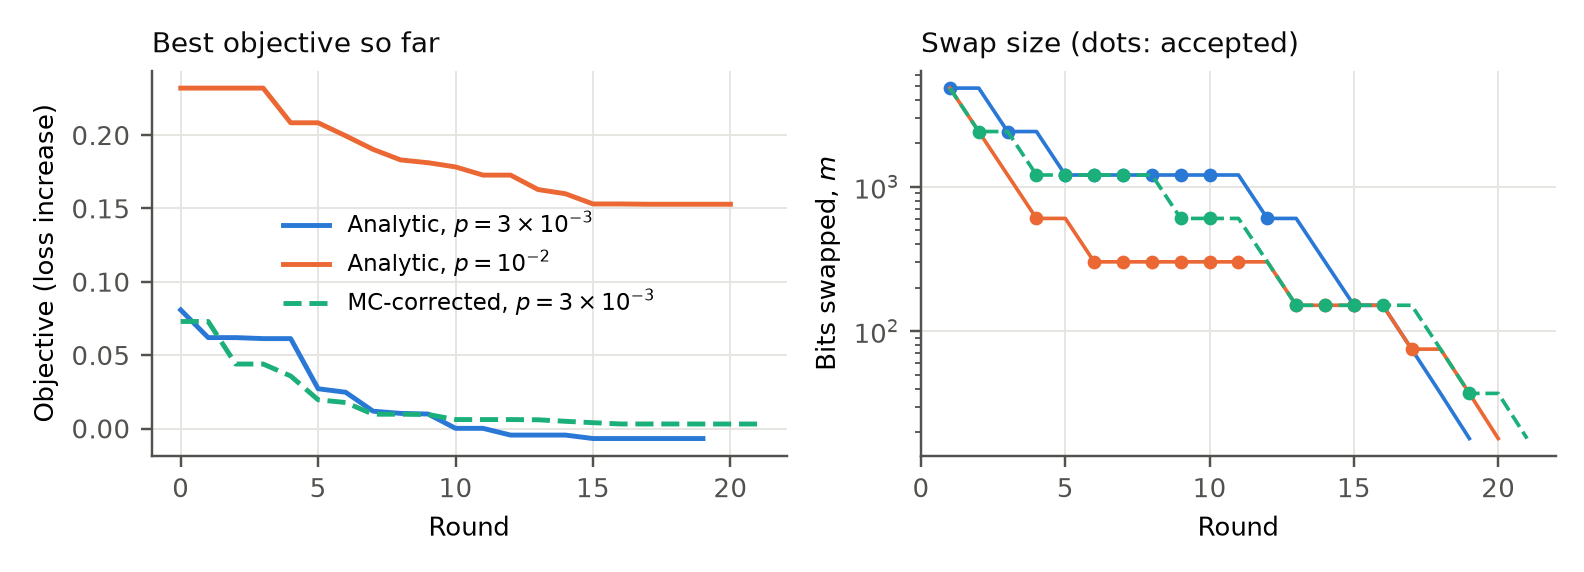
\includegraphics[width=\linewidth]{figures/runr_search_trace.png}
\caption{Course of the rate-aware search, pinned ResNet-8, replication 1, 12.5\% protection, held-out training images. Left: best objective found so far. Right: number of bits swapped per round; dots mark accepted rounds.}\label{fig:trace}
\Description{Objective and swap size per round of the rate-aware search at two bit-error probabilities, analytic and Monte Carlo corrected.}
\end{figure}

\paragraph{Predicted switch rates.} Table~\ref{tab:pstar} gives the frozen predictions of Stage~1 and Fig.~\ref{fig:switch-ckpt} compares them with the measurement for every checkpoint.

\begin{table}[h]
\caption{Predicted switch rate $p^*$ in units of $10^{-3}$, per checkpoint and budget, frozen before the Stage~1 fault fields were drawn. $^\dagger$At the end of the grid ($3\times10^{-2}$).}\label{tab:pstar}
\centering\small
\begin{tabular}{l r r r r r r r r}\toprule
Checkpoint & 1\% & 3.125\% & 6.25\% & 12.5\% & 18.75\% & 25\% & 37.5\% & 50\%\\\midrule
Pinned & 4.9 & 4.1 & 3.7 & 3.5 & 4.0 & 5.2 & 10.5 & 22.0\\
Seed 7101 & 3.3 & 2.8 & 3.3 & 3.1 & 3.6 & 4.9 & 9.0 & 19.4\\
Seed 7102 & 3.7 & 3.7 & 3.5 & 3.4 & 3.8 & 5.1 & 10.6 & 20.8\\
Seed 7103 & 4.1 & 3.5 & 3.3 & 3.2 & 3.9 & 5.2 & 10.6 & 22.0\\
Seed 7104 & 3.4 & 3.2 & 3.3 & 3.2 & 3.6 & 4.8 & 9.7 & 18.4\\
Seed 7105 & 1.6 & 2.6 & 2.4 & 2.6 & 3.2 & 4.5 & 8.8 & 18.4\\
Under-trained & 10.7 & 7.7 & 7.3 & 6.9 & 7.3 & 8.8 & 16.3 & 30.0$^\dagger$\\
Pruned 50\% & 5.4 & 4.9 & 4.8 & 4.8 & 4.9 & 6.0 & 10.5 & 19.2\\
Pruned 70\% & 3.7 & 4.2 & 3.7 & 3.2 & 3.1 & 3.3 & 5.0 & 8.4\\
\bottomrule
\end{tabular}
\Description{Predicted switch rates for nine ResNet-8 checkpoints at eight protection budgets.}
\end{table}

\begin{figure}[h]
\centering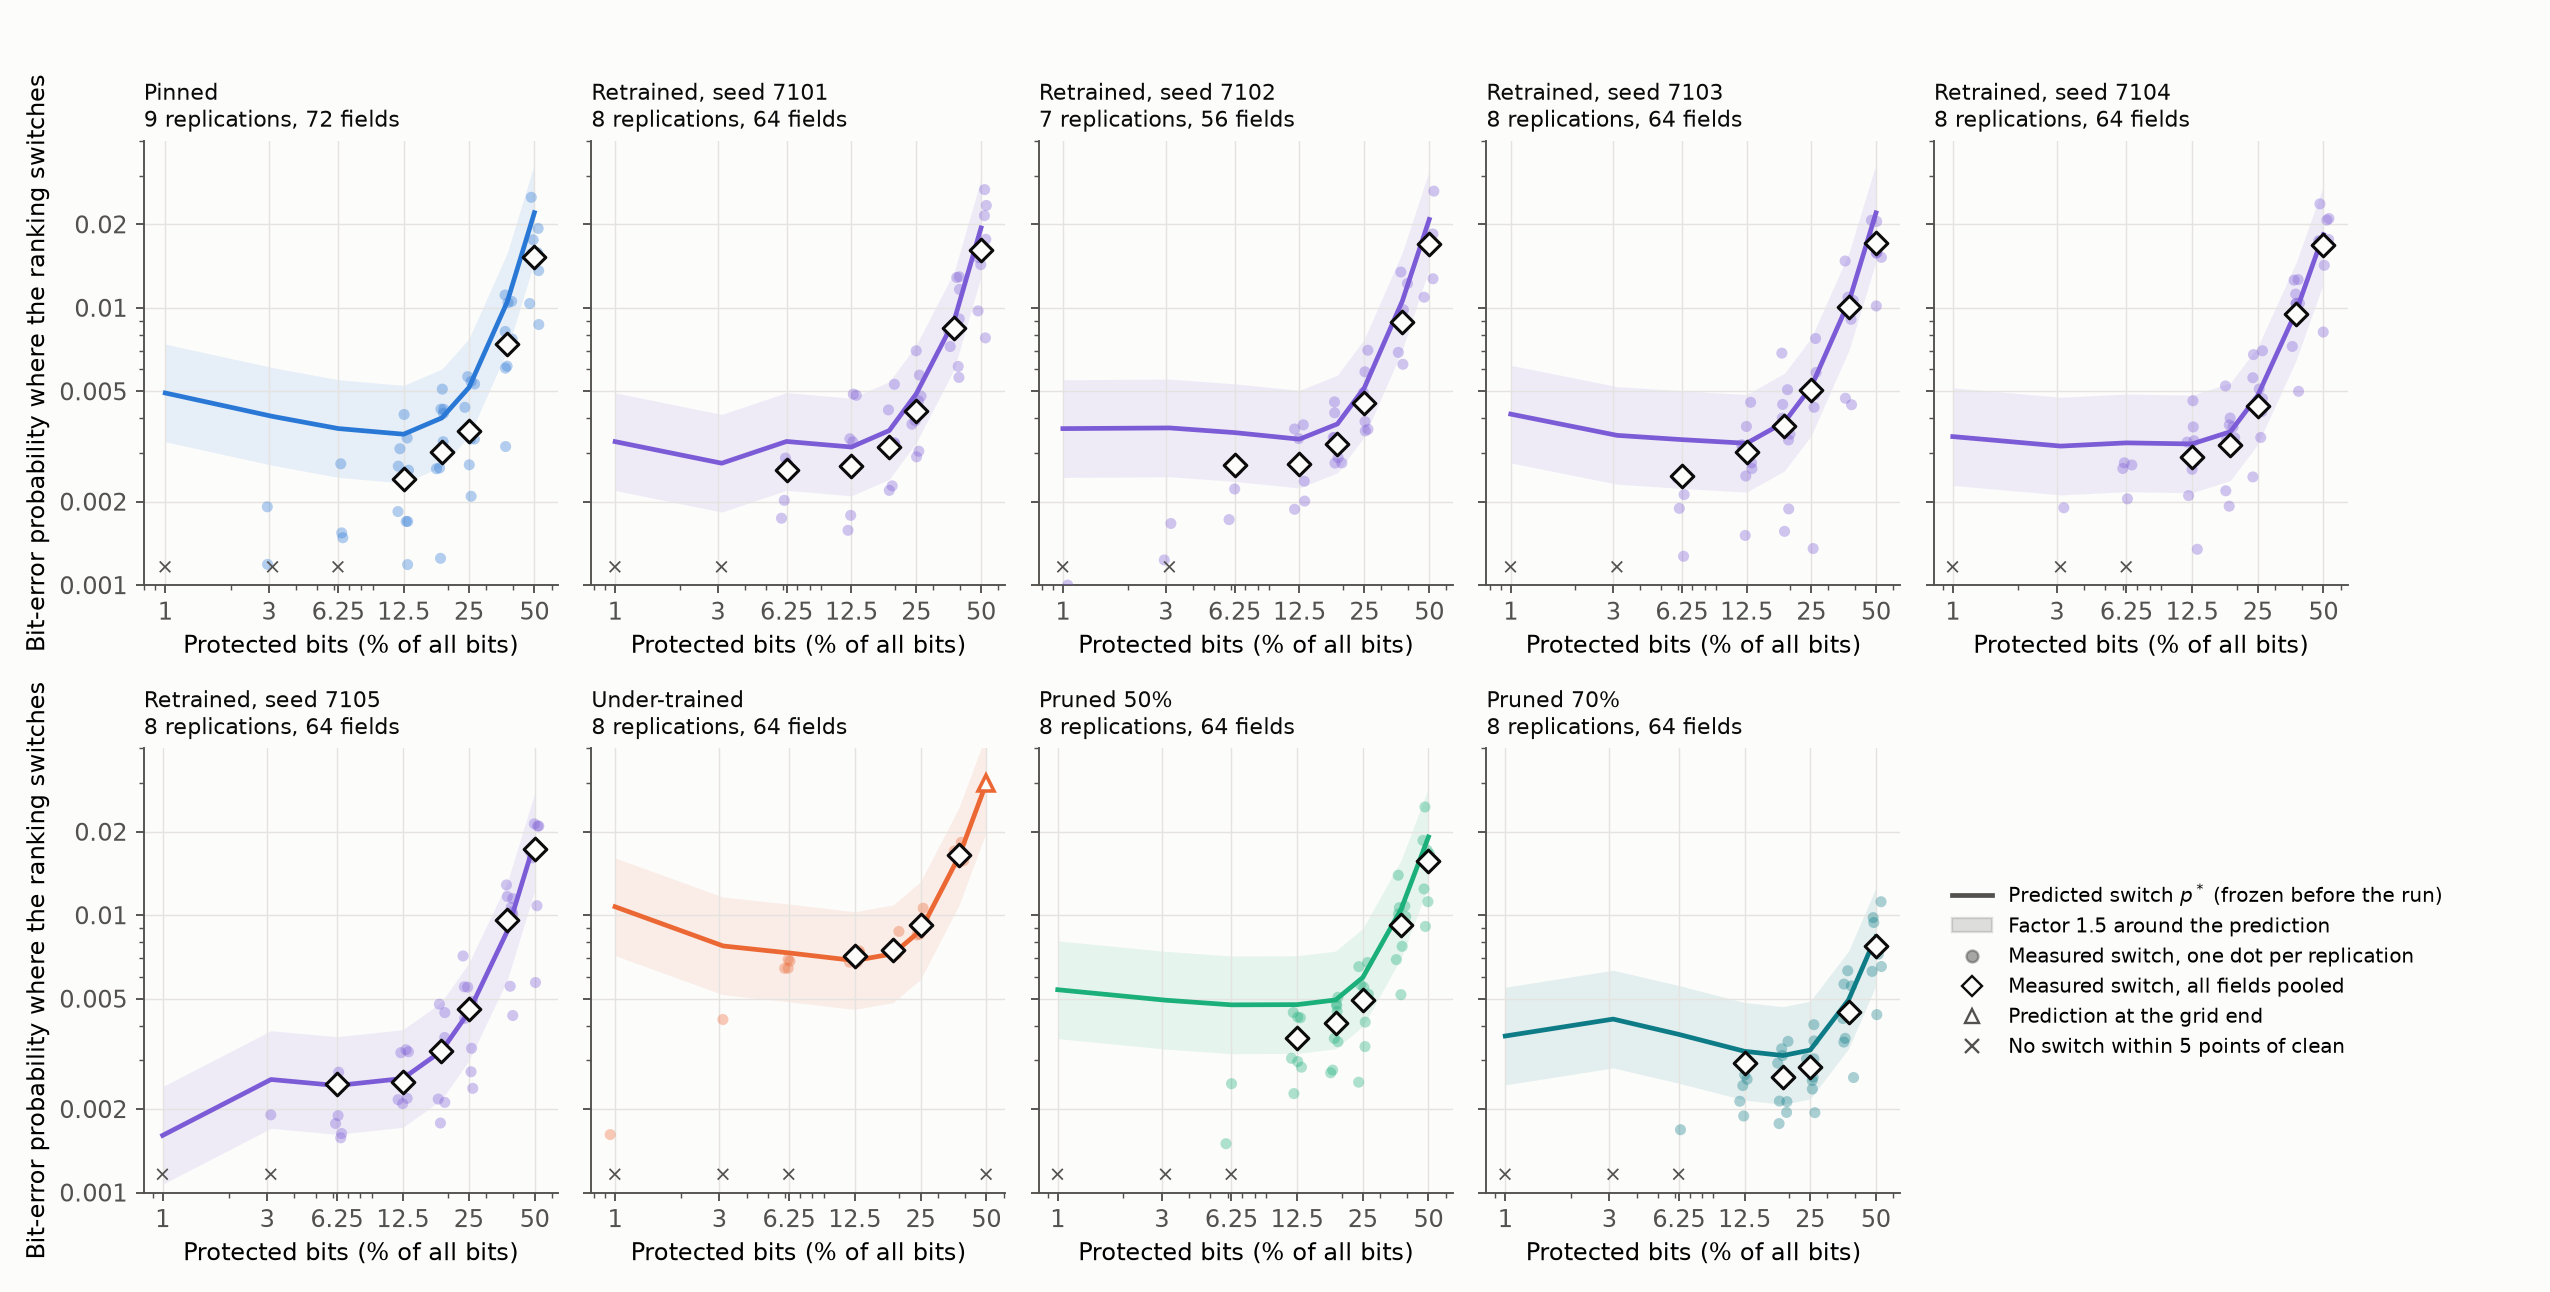
\includegraphics[width=\linewidth]{figures/stage1_switch_per_checkpoint.png}
\caption{Stage 1 per checkpoint: predicted switch (line, with the factor-1.5 band) against the share of protected bits, and the measured switch, per replication (dots) and with all fields pooled (diamonds). Crosses: no switch while the better mask stays within 5 points of clean.}\label{fig:switch-ckpt}
\Description{Nine panels of predicted and measured switch rate against protection budget.}
\end{figure}

\section{Execution, Identity and Surrogate Details}\label{app:implementation}
\subsection{Models, backends and eligible tensors}
Table~\ref{tab:identity} identifies the executed artifacts. The MLPerf Tiny models are the reference INT8 TFLite flatbuffers, executed with TensorFlow Lite 2.14.1 reference kernels; faults are XOR mutations of the INT8 kernel buffers in a private copy of the flatbuffer. The transformers are W8A8 executables derived from the public checkpoints. Every linear-layer weight matrix is stored as INT8 codes with one float32 scale per output channel, $s_i=\max_j|w_{ij}|/127$, rounding half to even, and codes in $[-127,127]$; the code $-128$ can arise only through a fault. Activations are quantized per token at run time, products accumulate exactly in INT32, and all other operations are float32. These are not integer-only networks. Every trial restores the clean state.

\begin{table}[h]
\caption{Executed artifacts. Hashes are SHA-256 prefixes of the model file or snapshot. ``Full-set'' is clean quality of the INT8 executable and its floating-point source on the complete evaluation split, which is larger than the cohort used under faults.}\label{tab:identity}
\centering\small
\begin{tabularx}{\linewidth}{l l X X}\toprule
Model & Source artifact & Eligible INT8 tensors & Full-set reference\\\midrule
ResNet-8 & MLPerf Tiny IC, \code{3c002613} & 10 kernels & cohort only\\
DS-CNN & MLPerf Tiny KWS, \code{aeea4368} & 10 kernels & cohort only\\
ToyCar & MLPerf Tiny AD, \code{87cf2419} & 10 kernels & cohort only\\
DistilBERT & SST-2 fine-tuned, rev. \code{714eb0fa}; \code{1f07e001} & 38 linear weights & 90.8\% vs 91.1\% (872 sentences)\\
Pythia-160M & rev. \code{b56d9bee}; \code{1264fe12} & 49 linear weights incl. output embedding & PPL 26.3 vs 25.4 (288,729 tokens)\\
Qwen3-0.6B & Base, rev. \code{da87bfb6}; \code{ea3fe5f6} & 197 linear weights incl. output head & PPL 12.5 vs 12.1 (299,077 tokens)\\\bottomrule
\end{tabularx}
\Description{Source artifacts, eligible tensors and full-set clean references for six models.}
\end{table}

Not faulted in any model: biases (INT32 in TFLite), quantization scales and zero points, and activations. Additionally not faulted in the transformers: input embedding tables, normalization parameters and the 42,242 to 496,000 per-channel scales. In the Qwen source model the output head is tied to the input embedding; the executable stores a separate quantized copy of the head, so a fault in the head does not alter the input embedding. The language-model cohorts are 4,096 scored tokens with clean perplexity 34.1 (Pythia) and 16.9 (Qwen), higher than the full-set values above.

\subsection{Exact jump and losses}
For affine decoding $w=s(q-z)$ and current stored bit value $a_j$, the exact INT8 jump is
\begin{equation}\label{eq:xor-delta}
\Delta w_j=\begin{cases}s(1-2a_j)2^j,&j<7,\\-s(1-2a_7)2^7,&j=7.\end{cases}
\end{equation}
The zero point cancels and each word keeps its own scale. TFLite cross-entropy is the mean of $-\ln\max\{(o+128)/256,10^{-12}\}$ over the cohort, with $o$ the INT8 output code of the true class, without renormalization; a per-example loss is therefore at most 5.5 nats or exactly 27.6 nats, and the mean is dominated by the count of zero-probability outputs, which is why classifier conclusions use accuracy. For ToyCar every window is evaluated under the same fault state, one score is formed per complete file, and ROC-AUC is computed over the 64 files with half credit for ties; reconstruction error is only the surrogate used for gradients. Transformer NLL is $\min\{\max(0,\mathrm{NLL}),30\}$ per sentence or token, with 30 assigned to nonfinite outputs; no nonfinite output occurred in any of the 9,984 saved language-model outcomes. The fraction of token losses that reach the cap was not recorded in the main grids and was obtained afterwards by replaying every saved fault field (Appendix~\ref{app:evidence}).

\subsection{Gradient and Hessian companions}
Gradient scores use a differentiable companion with straight-through requantization (TFLite) or the decoded weights with fixed float32 scales (transformers). The positive-part score is computed exactly from two saved moments, $\E_x\max(0,g)=\tfrac12(\E_x|g|+\E_x g)$ and $\E_x\max(0,-g)=\tfrac12(\E_x|g|-\E_x g)$, applied according to the sign of $\Delta_b$. The FKeras Hessian is that of a continuous float64 companion without activation rounding, using cross-entropy or ToyCar window MSE, two signed largest-magnitude eigenpairs, a Lanczos tolerance of $10^{-5}$ and 25 Hessian-vector products; normalized residuals are below $6.1\times10^{-16}$. These numbers certify the truncated continuous calculation, not a Hessian of the integer program. On 64 ResNet-8 inputs the continuous companion and the integer model agree on 61 predicted classes, with cross-entropy 0.626 against 0.918 nats.

\subsection{Tests in the source studies}
The finalized studies saved their own paired contrasts using sign-flip tests with $10^4$ random assignments and Holm families of 112 contrasts (TFLite, per BER and metric) and 160 contrasts (transformers, per model). Their smallest attainable adjusted $p$-values are therefore 0.0112 and 0.016. The analysis in this paper recomputes all contrasts from the saved field outcomes as described in Section~\ref{sec:experiments}.

\section{Fault-Model Motivation}\label{app:faultmotivation}
Only stored weights are faulted. Two published results motivate that choice and the range of $p$; neither calibrates it.

The first concerns exposure. In the architectural-vulnerability view, the error rate of a bit is its raw upset rate multiplied by the fraction of time during which it holds data that the computation still needs~\cite{mukherjee2003avf}; the same decomposition has been extended to delay faults caused by marginal defects~\cite{deutsch2024delayavf}. A stored weight is needed for the whole deployment, and an activation only until it is consumed. Li et al.\ quantified the consequence for the Eyeriss accelerator with one raw rate for all storage~\cite{li2017understanding}. The projected failure rate of the filter memory is 3.0 FIT for AlexNet and 3.9 FIT for NiN. The global buffer, which holds the feature maps passed between layers, contributes 0.20 and 0.04 FIT, the image and partial-sum registers at most 0.006 FIT, and the whole datapath of NiN 0.004 FIT. The authors give two reasons: buffers are larger than the datapath, and a stored fault is read many times. Tyagi et al.\ make the same point for vulnerability estimation, arguing that the weights and activations of an accelerator should not be assumed to have equal fault probability~\cite{tyagi2023thales}. The same study marks the limit of the argument. For its smallest network the global buffer (87.5 FIT) exceeds the filter memory (62.7 FIT). Which storage dominates is therefore a property of the architecture and of how long values are held. We study stored weights because they are the persistent state of an accelerator, and we do not claim that weight faults are always the more important ones.

The second concerns magnitude. Proton-beam tests of ECON-D, a radiation-hard front-end ASIC of the CMS high-granularity calorimeter, report an upset cross section of a few $10^{-14}$\,cm$^2$ per flip-flop before voting, and the chips were tested to a fluence of $5\times10^{13}$ protons per cm$^2$~\cite{cummings2023econd}. As an illustration only: if a hadron fluence of order $10^{13}$--$10^{14}$\,cm$^{-2}$ accumulates over the roughly $6\times10^{7}$\,s of beam that 3000\,fb$^{-1}$ at $5\times10^{34}$\,cm$^{-2}$\,s$^{-1}$ require~\cite{hllhc2017tdr}, a register bit with that cross section that is neither protected nor rewritten accumulates an upset probability of order $10^{-5}$ to $10^{-4}$ per hour of beam; it reaches $10^{-3}$ within hours to days and $10^{-2}$ within days to weeks, which spans the band in which the masks of this study differ. A value held for one 25\,ns bunch crossing sees about $10^{-11}$ of the hourly figure. These chips triplicate their registers for this reason, and the neural-network encoder of the same detector keeps its weights in triplicated, self-correcting registers~\cite{diguglielmo2021reconfigurable}. The question studied here is what is lost when less than everything is protected. The numbers come from one technology and one environment, and the cross section is read from a published plot; $p$ remains a model parameter.

\section{Repeated Evaluations: Curves and Partial Tiers}\label{app:repeated}
Figure~\ref{fig:confirm} shows the repeated evaluation of the two pinned classifiers. A first DS-CNN run with three replications agreed in its estimates (largest regret 0.13 points, no resolved loss), but its replication-level bounds, with a Student-$t$ quantile of 4.3, exceeded one point in eight cells; the second run with eleven replications meets the rule. The DS-CNN windows had also been used by earlier six-bit conditional-selection studies, though not for whole-mask comparisons, and we did not audit whether a 200-image subset used in early ResNet-8 engineering runs overlaps the new ResNet-8 windows.

\begin{figure}[tbp]
\centering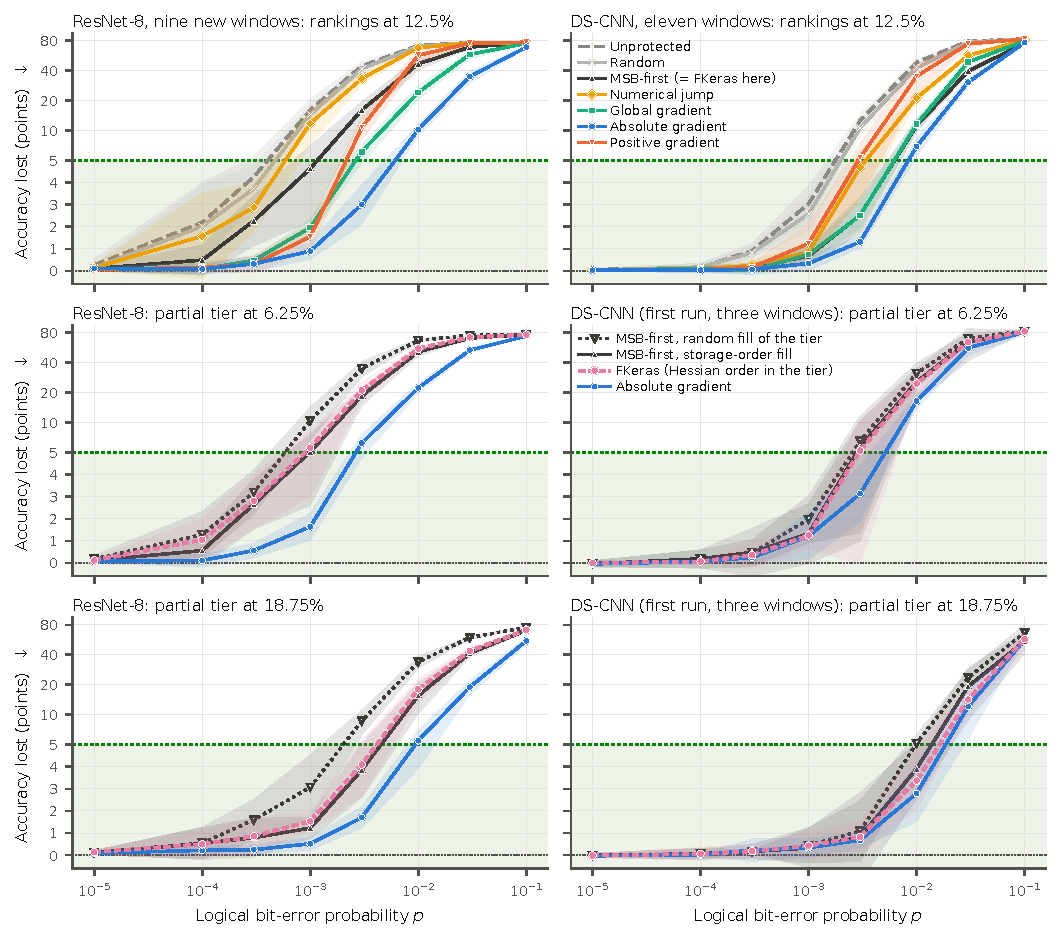
\includegraphics[width=\linewidth]{tecs_confirmation_runA}
\caption{Repeated evaluation of the pinned checkpoints on other input windows. Accuracy lost against each replication's clean accuracy; bands are 95\% intervals over replications (nine for ResNet-8, three for DS-CNN in this run) and the shaded region is the usefulness margin. The vertical axis is linear up to five points and logarithmic above. Top: the seven rankings at 12.5\% protection, where FKeras selects the same mask as MSB-first. Middle and bottom: the two partial-tier budgets, where the half-protected tier is filled by tensor storage order, by the FKeras Hessian order, or uniformly at random (mean of four fills).}\label{fig:confirm}
\Description{Six panels of accuracy lost against bit-error probability for ResNet-8 and DS-CNN on new evaluation windows.}
\end{figure}

\begin{figure}[tbp]
\centering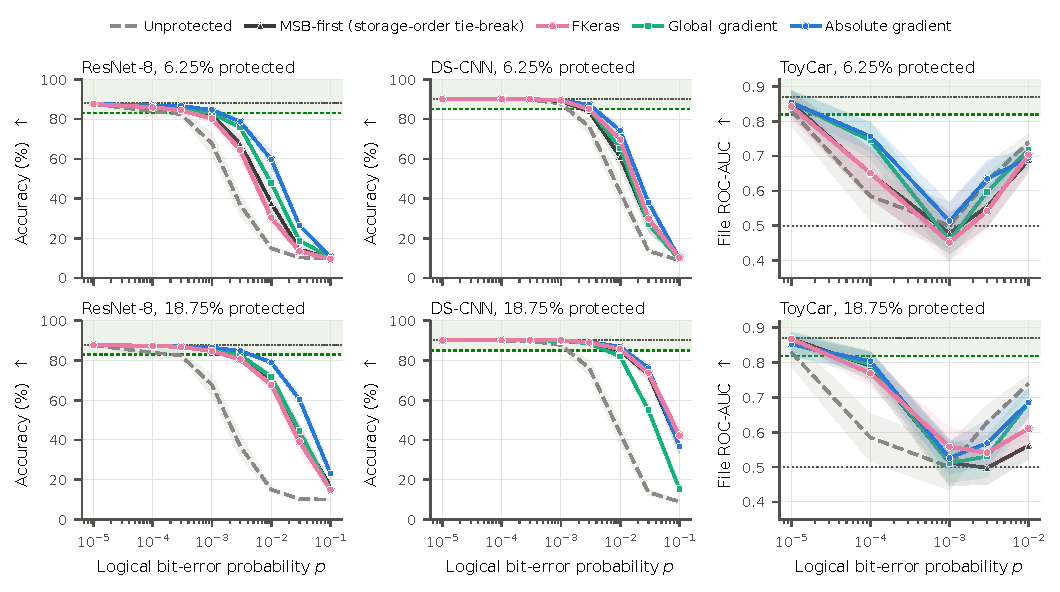
\includegraphics[width=\linewidth]{tecs_fkeras_partial_tiers}
\caption{FKeras at the two partial-tier budgets, where its mask differs from MSB-first, on the three models for which it was measured. Bands are 95\% intervals of the field mean; the shaded region is the usefulness margin. MSB-first here resolves the half-protected tier by tensor storage order.}\label{fig:fkeras}
\Description{Six panels comparing FKeras with MSB-first, global gradient and absolute gradient at 6.25 and 18.75 percent protection.}
\end{figure}

Contrasts between FKeras and MSB-first at the partial tiers (Fig.~\ref{fig:fkeras}) need a reference, because the MSB-first mask there is determined by tensor storage order (Section~\ref{sec:susceptibility}), so the repeated evaluations included four masks that fill the partial tier uniformly at random (Fig.~\ref{fig:confirm}, middle and bottom). Both structured fills are better than the random one. On ResNet-8 the random fill has a resolved higher error rate than FKeras in 9 of the 16 partial-tier cells and than the storage-order mask in 12, by up to 16.0 and 18.4 points at $p=10^{-2}$ and 18.75\%, and by 4.9 and 5.4 points at $p=10^{-3}$ and 6.25\%, inside the useful region. On DS-CNN the counts are 4 and 5 cells. FKeras is nevertheless not better than plain storage order. No difference between the two is resolved in a decision-useful cell of either model, where they differ by at most 0.6 points, and on ResNet-8 at $p=10^{-2}$ the storage-order mask is better by 4.0 points at 6.25\% (replication-level interval 2.2 to 5.8) and by 2.5 points at 18.75\%. Storage order protects complete tensors, beginning with the first layers; we did not test whether that explains its advantage over a uniform fill.

\section{Calibration Size of the Gradient Rankings}\label{app:calibration}
Every other comparison builds its masks from 64 calibration inputs. For each replication of the nine ResNet-8 checkpoints of Table~\ref{tab:repeated} we rebuilt the absolute-, positive- and global-gradient masks from the first 128, 256, 512 and 1,024 training images of the block that begins with the replication's own 64, at the bit counts of the saved masks, and replayed them on the replication's saved fault fields and input window at $p=10^{-3}$, $3\times10^{-3}$, $10^{-2}$ and $3\times10^{-2}$ (28,512 new evaluations; the 1,024-input set overlaps the next replication's first 24 inputs). Before any evaluation each rebuilt 64-input mask had to agree with the saved one in at least 99.9\% of its bits, and every saved fault field had to reproduce the saved outcome of one saved mask exactly; all 648 did. One replication of the retrained copy R2 failed the first check (99.66\% to 99.92\%: its saved masks came from gradients about 1\% different from those recomputed now) and was excluded before any outcome. Two rules were fixed before the runs, each tested with pooled-field sign-flip tests and Holm correction over its 328 contrasts. The default holds if neither the positive nor the global gradient, built from 512 or 1,024 inputs, is resolved ahead of the absolute gradient built from the same inputs by half a point or more in a decision-useful cell where it was not already resolved ahead with 64. Calibration size matters for the default if its 512- or 1,024-input mask is resolved ahead of its 64-input mask by half a point on at least three checkpoints.

\begin{table}[tbp]
\caption{Positive- minus absolute-gradient mask, both built from the same number of calibration inputs, in the decision-useful cells of the nine ResNet-8 checkpoints (accuracy points). Ahead: cells where the positive-gradient mask has the higher mean accuracy. Resolved: Holm-corrected sign-flip tests; the 64-input row uses the masks of Table~\ref{tab:repeated}.}\label{tab:calibration}
\centering\footnotesize
\begin{tabular}{l r r r r c c}\toprule
BER & Inputs & Cells & Ahead & Median & Range & Resolved ahead / behind\\\midrule
$10^{-3}$ & 64 & 36 & 17 & $-0.01$ & $-0.81$ to $+1.30$ & 4 / 1\\
 & 512 & 36 & 36 & $+0.65$ & $+0.23$ to $+1.32$ & 8 / 0\\
 & 1,024 & 36 & 36 & $+0.65$ & $+0.24$ to $+1.55$ & 9 / 0\\\midrule
$3\times10^{-3}$ & 64 & 29 & 3 & $-4.29$ & $-8.10$ to $+1.46$ & 0 / 22\\
 & 512 & 29 & 15 & $+0.17$ & $-1.28$ to $+2.41$ & 4 / 0\\
 & 1,024 & 29 & 20 & $+0.42$ & $-0.91$ to $+2.46$ & 5 / 0\\\midrule
$10^{-2}$ & 64 & 15 & 0 & $-36.9$ & $-46.4$ to $-12.3$ & 0 / 15\\
 & 512 & 15 & 0 & $-10.2$ & $-22.6$ to $-0.5$ & 0 / 13\\
 & 1,024 & 15 & 0 & $-8.1$ & $-17.8$ to $-0.6$ & 0 / 12\\\midrule
$3\times10^{-2}$ & 1,024 & 2 & 0 & $-54.6$ & $-58.3$ to $-50.8$ & 0 / 2\\\bottomrule
\end{tabular}
\Description{Counts, medians and ranges of the accuracy difference between positive- and absolute-gradient masks at three calibration sizes and four bit-error probabilities.}
\end{table}

The first rule fails (Table~\ref{tab:calibration}). The positive-gradient mask is resolved ahead by 0.5 to 2.5 points in ten cells on five checkpoints: five cells of the under-trained checkpoint at $10^{-3}$ and $3\times10^{-3}$ and one or two cells at those rates on the 50\%-pruned checkpoint and on R1, R3 and R4. With 1,024 inputs, resolved wins in both directions appear on the pinned checkpoint (three ahead at $10^{-3}$, one behind at $10^{-2}$), the under-trained one (8 and 3), the 50\%-pruned one (1 and 1), R1 and R4 (1 and 2 each). The global gradient is never ahead. Its mask keeps changing with more inputs (the 512-input mask shares 80\% to 87\% of its bits with the 1,024-input mask at 12.5\%, against 94\% to 96\% for the positive and 96\% to 97\% for the absolute gradient), but its accuracy does not improve: averaging signed effects over more inputs converges to a mean gradient that is small for a trained model. The second rule is not met. In the 82 decision-useful cells the absolute-gradient mask gains a median 0.09, 0.15, 0.20 and 0.23 points from 128, 256, 512 and 1,024 inputs, at most 1.5, with a single resolved gain of 0.44 points; going from 512 to 1,024 inputs changes it by a median 0.06. Pooled over the five retrained copies, however, its 1,024-input mask gains 0.95 and 0.55 points at $p=10^{-2}$ and 18.75\% and 25\% protection (95\% intervals over copies 0.74 to 1.16 and 0.19 to 0.90), so at the densest useful rates a larger calibration set is worth about half a point to a point. At $p=10^{-3}$ and 25\%, the 512-input positive-gradient mask leaves seven of the eight well-trained checkpoints at or above their clean accuracy, by up to 0.64 points, and the under-trained one 1.0 point above, whereas the 1,024-input absolute-gradient mask leaves six of the nine slightly below. This is the low-rate side of the mechanism of Section~\ref{sec:harm}; it was not tested, and 0.1 point is one image of the 1,000-image window. Rates below $10^{-3}$, other models and FKeras were not measured at larger calibration sizes.

\section{Protection Worse Than None: Checks and Mechanism}\label{app:harm}
Before treating the harm of Section~\ref{sec:harm} as an effect we checked it as a possible defect. The ranking code computes $\E_x\max(0,e_b(x))$ exactly from the saved mean and mean-absolute gradients and from the exact XOR jump of each stored code. Fields are paired by hash; in every saved outcome the proposed count equals applied plus suppressed, and no protected run applies more faults than its unprotected partner. No nonfinite output occurred, so the failure penalty plays no role. The low-BER behaviour is also what a correct sign predicts: where faults are sparse, the positive-gradient mask is the best ranking on the two language models and within 0.2 accuracy points of the best on DistilBERT. On Pythia, in the four cells at $p=3\times10^{-3}$ where the positive-gradient mask has a higher loss than no protection, at most 6\% of token losses are capped and the uncapped difference is 1.1 to 5.5 nats per token.

\begin{table}[t]
\caption{DistilBERT, 12.5\% protection. First-order effect of the faults left unprotected, split into loss-increasing and loss-decreasing parts and summed over bits (the predicted mean loss change is $p$ times the net value). Jump energy is $\sum\Delta_b^2$ over unprotected bits relative to no protection. Accuracy is measured at $p=10^{-2}$.}\label{tab:drift}
\centering\small
\begin{tabular}{l r r r r r}\toprule
Mask & Increasing & Decreasing & Net & Jump energy & Accuracy (\%)\\\midrule
Unprotected & $+32.94$ & $-32.86$ & $+0.08$ & 1.00 & 60.3\\
Random & $+28.82$ & $-28.75$ & $+0.07$ & 0.87 & 62.3\\
MSB-first & $+16.35$ & $-16.42$ & $-0.07$ & 0.25 & 87.6\\
Numerical jump & $+16.52$ & $-16.48$ & $+0.04$ & 0.16 & 89.5\\
Global gradient & $+8.55$ & $-8.54$ & $0.00$ & 0.39 & 90.0\\
Absolute gradient & $+10.41$ & $-10.41$ & $0.00$ & 0.33 & 90.7\\
Positive gradient & $+6.67$ & $-20.62$ & $-13.95$ & 0.37 & 58.5\\\bottomrule
\end{tabular}
\Description{Residual first-order effect, jump energy and measured accuracy for seven DistilBERT masks.}
\end{table}

Table~\ref{tab:drift} gives the mechanism, obtained offline from the saved gradients, masks and stored codes of DistilBERT. For every other mask the loss-increasing and loss-decreasing first-order effects of the unprotected bits cancel to within 0.5\%. The positive-gradient mask protects mainly flips predicted to increase the loss (72\% of its protected bits, against 50\% for the others) and so leaves a one-sided remainder: $+6.7$ against $-20.6$. A first-order model would then predict that faults reduce the loss by $0.14$ nats at $p=10^{-2}$, which is impossible for a model whose loss is already near its minimum on the calibration set. The many remaining faults push the weights coherently in one direction, far beyond the range in which a gradient describes the loss, and the measured loss rises instead. The amount of perturbation left is not the explanation: the positive-gradient mask leaves about the same jump energy as the absolute- and global-gradient masks (0.37 against 0.33 and 0.39).

The stored codes of the under-trained ResNet-8 are distributed like those of the pinned model and of the five retrained copies: mean magnitude 31.9 code units against 31.4 and 31.3 to 31.9, and 15.6\% of codes below 8 in magnitude against 15.9\% and 15.5\% to 16.1\%.

Two weaker cases should not be confused with this one. MSB-first has a higher loss than the unprotected DistilBERT model in four cells at $p\ge3\times10^{-2}$ but never a lower accuracy: the model becomes more confidently wrong, not more often wrong. And at $p=10^{-1}$ several ResNet-8 masks have a higher cross-entropy than no protection although their accuracy is above, or within 0.2 points of, the unprotected model's 10\%. That ordering is produced by the loss floor, not by the task.

\section{Conditional Evaluation}\label{app:proofs}
Exact local re-selection does not help measurably in the one setting we could test. On DS-CNN at $p=5\times10^{-2}$, in 32 randomly drawn pools of six bits, two protected and four unprotected under the 12.5\% absolute-gradient mask, we re-chose which two bits of each pool to protect, using isolated or background-conditioned measured damage. The two selectors differ on held-out fields by $-8\times10^{-5}$ nats per clip (interval $-0.0017$ to $0.0015$), and each improves on the original mask by about $0.003$ nats per clip. At that BER the model is not useful (background loss 7.1 nats per clip), the whole range of risk across the 15 possible masks of a pool has a median of 0.013 nats per clip, and the selected mask beats its runner-up by less than two paired standard errors in all 32 pools. The study shows that re-selecting two of six random bits cannot matter much; it does not show whether conditional information helps a selector with a useful search space.

\subsection{Protection benefit and paired swaps}
Conditioning on whether unprotected bit $b$ flips gives $J_p(\protset)=(1-p)\E\risk(G)+p\E\risk(G\cup\{b\})$. Protecting it leaves $\E\risk(G)$, which proves Eq.~\eqref{eq:protection-benefit}. Under additive risk the best exact-budget mask protects the bits with the largest isolated effects; nonadditive risk need not preserve that order. For a swap that exposes protected bit $a$ and protects unprotected bit $b$, giving mask $\protset'$, a common background $G$ that excludes both bits and all protected coordinates gives
\begin{equation}\label{eq:swap}
J_p(\protset')-J_p(\protset)=p\,\E_G[\risk(G\cup\{a\})-\risk(G\cup\{b\})].
\end{equation}
Both identities hold for any scalar risk, including complete-cohort AUC, under independent faults; they do not hold for correlated or fixed-count fault laws.

\subsection{The 32-pool DS-CNN study}
Each pool $C$ contains six bits, two protected and four unprotected in the 12.5\% absolute-gradient mask, drawn uniformly within those two strata. All other protected bits stay fixed. For each of eight selection fields on the bits outside the pool, the model is evaluated in all $2^6$ fault states of the pool, giving the exact conditional risk of each of the 15 two-bit masks $Q$,
\begin{equation}\label{eq:response-table}
J_G(Q)=\sum_{A\subseteq C\setminus Q}p^{|A|}(1-p)^{|C\setminus Q|-|A|}\,\risk(G\cup A).
\end{equation}
Conditional selection takes the mask with the lowest mean $J_G$; isolated selection protects the two bits with the largest clean isolated damage. The three masks (original, isolated, conditional) are then compared on 32 new fields and 384 clips using Eq.~\eqref{eq:swap}. The pool is the unit of inference.

\begin{figure}[h]
\centering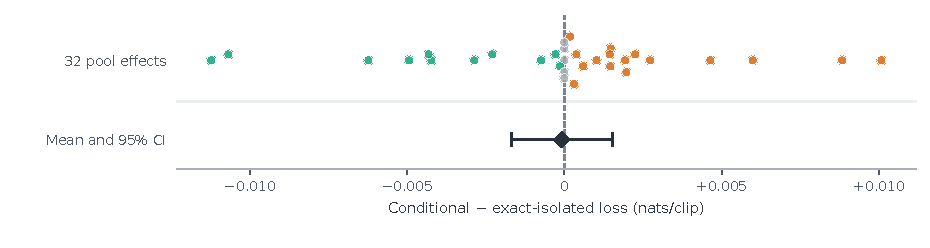
\includegraphics[width=.85\linewidth]{compact_kws_pools}
\caption{Held-out conditional-minus-isolated loss in the 32 DS-CNN pools at $p=5\times10^{-2}$, with the mean and its 95\% pool-level interval. Negative favours conditional selection. The background loss is about 7 nats per clip.}\label{fig:decisions}
\Description{Thirty-two pool effects scattered around zero with an unresolved mean.}
\end{figure}

The held-out means are $-0.00268$ nats per clip for conditional against original (interval $-0.00478$ to $-0.00058$), $-0.00248$ for isolated against original ($-0.00459$ to $-0.00036$) and $-0.00008$ for conditional against isolated ($-0.00169$ to $0.00153$; Fig.~\ref{fig:decisions}). The three do not add up exactly because each contrast is estimated along its own swap path with its own analytically integrated coordinates; the estimands are transitive, the finite estimates are not, and 15 of the 32 pools are exactly transitive. On the selection tables, the range of risk over the 15 masks has a median of 0.013 and a maximum of 0.086 nats per clip, and the selected mask leads its runner-up by a median of 0.0009. The in-sample advantage of the conditional mask over the isolated one is 0.0053, against 0.00008 held out. Candidate bits are spread over all positions, with 46 sign bits and 17 least-significant bits among the 192. Earlier counts of how often an additive prediction misorders masks on the selection tables are not reported, because the conditioned predictor and its target share the same sampled fields.

\section{Supplementary Measurements}\label{app:evidence}
\begin{figure}[h]
\centering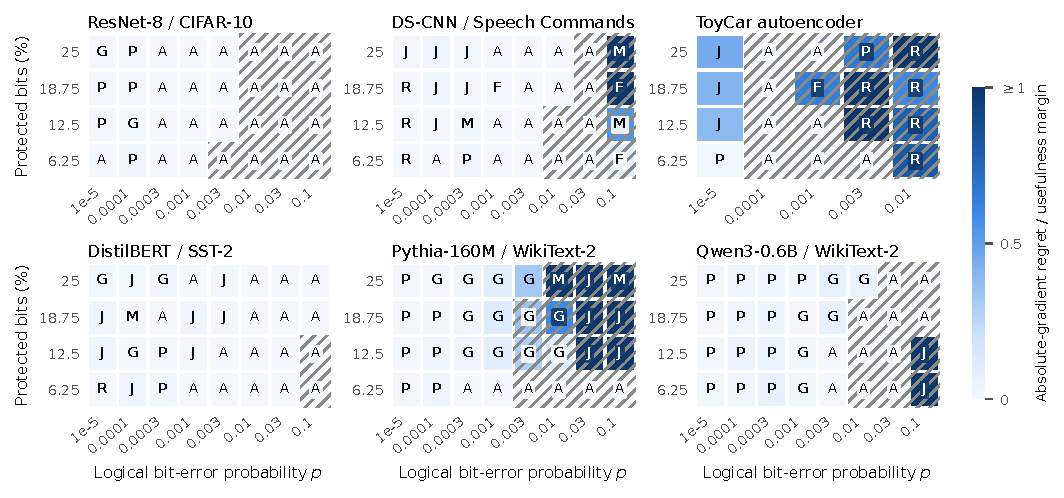
\includegraphics[width=\linewidth]{tecs_grid_regret_map}
\caption{The complete grid. Colour: regret of the absolute-gradient mask divided by the usefulness margin (0.05 accuracy or AUC, 0.5 nats/token). Letter: best measured ranking in the cell (A absolute, G global, P positive gradient, M MSB-first, F FKeras, J numerical jump, R random); bold when it is not absolute gradient. Hatched cells are not decision-useful.}\label{fig:map}
\Description{Six heat maps over bit-error probability and budget showing absolute-gradient regret and the best ranking per cell.}
\end{figure}

Of the 32 cells per model, 19 (ResNet-8), 22 (DS-CNN), 30 (DistilBERT), 17 (Pythia) and 21 (Qwen) are decision-useful, and in 11, 6, 14, 9 and 9 of them the unprotected model is not. Once the ToyCar autoencoder is heavily corrupted, file AUC reflects how the corrupted model orders files rather than preserved function, so its AUC at high BER is not interpreted.

\begin{table}[h]
\caption{Spearman correlation with positive isolated damage on 320 stratified candidate bits per model, with 95\% within-stratum bootstrap intervals. These are sample-design statistics, not whole-network correlations. ToyCar AUC values are descriptive. FKeras entries for DS-CNN and ToyCar were not computed because the calibration inputs of the saved candidate audit and of the Hessian scores could not be matched.}\label{tab:isolated}
\centering\small
\begin{tabular}{l l l l r}\toprule
Ranking & ResNet-8 & DS-CNN & ToyCar (MSE) & ToyCar (AUC)\\\midrule
Random & $-0.05$ [$-0.15$, 0.04] & 0.01 [$-0.08$, 0.10] & 0.06 [$-0.04$, 0.15] & 0.03\\
MSB-first & 0.26 [0.17, 0.34] & 0.20 [0.11, 0.28] & 0.50 [0.43, 0.57] & 0.32\\
Numerical jump & 0.07 [$-0.02$, 0.16] & 0.17 [0.08, 0.26] & 0.44 [0.36, 0.51] & 0.23\\
Global gradient & 0.36 [0.29, 0.45] & 0.26 [0.16, 0.35] & 0.50 [0.41, 0.58] & 0.49\\
Absolute gradient & 0.38 [0.29, 0.46] & 0.29 [0.20, 0.38] & 0.55 [0.46, 0.63] & 0.50\\
Positive gradient & 0.36 [0.28, 0.45] & 0.25 [0.16, 0.33] & 0.64 [0.56, 0.71] & 0.50\\
FKeras & 0.29 [0.21, 0.37] & --- & --- & ---\\\bottomrule
\end{tabular}
\Description{Rank correlations of seven scores with measured isolated damage on three models.}
\end{table}

\paragraph{Single-fault fidelity and cost.} Single-fault fidelity does not predict protection quality. On 320 stratified candidate bits per TFLite model, Spearman correlations between each score and the measured positive isolated damage are low to moderate (Table~\ref{tab:isolated}): 0.07 (numerical jump) to 0.38 (absolute gradient) on ResNet-8 and 0.17 to 0.29 on DS-CNN, with bootstrap intervals of about $\pm0.09$ that overlap among the three gradient scores. Global, absolute and positive gradient have nearly equal correlations on ResNet-8 (0.36, 0.38, 0.36), yet their worst accuracy regrets differ (2.1, 0.06 and 3.2 points). Score construction is cheap for the small models. Mean times on ResNet-8, DS-CNN and ToyCar are 1.2, 0.4 and 3.8 seconds for the global gradient, 17, 7.5 and 208 seconds for the shared per-example gradients behind the absolute and positive scores, and 5.6, 1.4 and 11.4 seconds for the rank-two Hessian projection. MSB-first needs no data. Score-construction times for the transformers were not recorded; one evaluation of a faulted transformer took a median of 12 to 33 seconds.

\paragraph{ToyCar.} ToyCar behaves differently and cannot inform the choice of ranking. Its unprotected mean AUC falls from 0.83 at $p=10^{-5}$ (about 21 faults) to 0.50 at $10^{-3}$ and then rises again to 0.74 at $10^{-2}$; a single field at $10^{-5}$ gives 0.34. Once the autoencoder is heavily corrupted, file AUC reflects how the corrupted model happens to order files, not preserved function. Only the four cells at $p=10^{-5}$ are decision-useful, the unprotected model is useful in all of them, and no contrast between rankings is resolved there.

\paragraph{Loss cap.} A replay of every saved language-model fault field, reproduced bit for bit, shows where the cap matters. No token is capped in the useful conditions of Qwen and one in those of Pythia, and removing the cap changes neither the best ranking nor the absolute-gradient regret in any decision-useful cell. Outside the useful region the cap dominates on Pythia, where 18\% of the unprotected model's token losses are capped at $p=10^{-2}$ and 83\% at $3\times10^{-2}$, against 1\% and 9\% on Qwen. Without the cap the best ranking would change in two Pythia cells, both at $p\ge3\times10^{-2}$; capped losses there are lower bounds on the damage.

\paragraph{Comparisons outside the useful region.} For completeness we record two comparisons that the previous version of this work emphasized and that lie where no ranking keeps the model useful. On Pythia at $p=10^{-2}$, global gradient minus MSB-first is $-4.82$ nats per token at 12.5\% protection and $+0.77$ at 25\%. In a separate exploratory run on Qwen with 24 new fields per BER, absolute gradient minus MSB-first at 12.5\% is $-9.30$ nats per token at $p=5\times10^{-2}$ (interval $-10.02$ to $-8.57$) and $+1.64$ at $7.5\times10^{-2}$ ($0.61$ to $2.66$); at the latter BER 10.5\% and 7.1\% of finite token losses reach the cap for the two masks and the mean losses exceed 21 nats per token. Two focused runs with more fields give, on ResNet-8 at $p=10^{-2}$ and 6.25\%, FKeras minus MSB-first cross-entropy of $+2.24$ nats per image (320 fields, interval $1.89$ to $2.59$), and on ToyCar at $p=10^{-2}$ and 18.75\%, FKeras minus absolute-gradient risk of $+0.111$ (384 fields, $0.092$ to $0.129$). None of these bears on the conclusions of the paper.

\section{Search-Based, Relaxed and Literature-Derived Masks}\label{app:search}
To test whether optimizing the mask beats a fixed ranking, we built five further kinds of mask for the pinned ResNet-8 at 12.5\% and 25\% protection, from the 64 calibration images of one repeated-evaluation replication (training images 2000--2063), and evaluated them with the TFLite executable on test images 2000--2999 under 16 common fault fields per rate. Search objectives used 256 further training images (27000--27255).
\begin{itemize}
\item \emph{MC-guided swap search.} Starting from the absolute-gradient mask, each of eight rounds samples fault fields under the current mask, re-scores bits by the mean per-example absolute gradient of the faulted models, proposes three swap sets towards the re-scored top bits, and keeps a proposal only if it lowers the validation loss on twelve common fault fields. One mask per rate.
\item \emph{Relaxed per-bit optimization.} A protection probability per bit is optimized with Adam: each step samples a fault field, scales every sampled fault by one minus its bit's protection probability in the differentiable companion, and restores the budget; the final mask protects the top bits. This is a pathwise-gradient relative of policy-gradient reinforcement learning. One mask per rate, and one with the rate drawn log-uniformly from $[3\times10^{-3},3\times10^{-2}]$ at every step.
\item \emph{Group CEM.} The cross-entropy method over 80 groups (10 kernel tensors $\times$ 8 bit positions); whole groups are filled in sampled order and the last group in absolute-gradient order, so the mask is regular by construction.
\item \emph{Thales.} Bits ranked by their single-flip accuracy loss on the calibration images, ties broken by cross-entropy increase, from an exhaustive table of all 618,880 single flips; our adaptation of the Thales vulnerability factor with a uniform fault probability~\cite{tyagi2023thales}.
\item \emph{HarDNN.} Output filters ranked by the mean absolute loss change of their bits, or by their mean per-example absolute gradient (HarDNN's best cheap heuristic), and protected whole~\cite{mahmoud2020hardnn}.
\end{itemize}
\begin{table}[h]
\caption{Pinned ResNet-8, test images 2000--2999 (clean accuracy 85.6\%), 16 common fault fields per rate. First row: accuracy of the absolute-gradient mask; other rows: paired difference from it, in points; bold when the 95\% field-level interval excludes zero (no multiplicity correction). Masks built for one rate are evaluated at that rate. The first three cells are usable (within five points of clean).}\label{tab:search}
\centering\footnotesize\setlength{\tabcolsep}{4pt}
\begin{tabular}{l r r r r r r}\toprule
BER & $3\!\times\!10^{-3}$ & $3\!\times\!10^{-3}$ & $10^{-2}$ & $10^{-2}$ & $3\!\times\!10^{-2}$ & $3\!\times\!10^{-2}$\\
Protection & 12.5\% & 25\% & 25\% & 12.5\% & 12.5\% & 25\%\\\midrule
Absolute gradient (accuracy, \%) & 83.0 & 85.0 & 83.7 & 76.8 & 54.1 & 79.7\\
MC-guided swap search & +0.1 & $-$0.1 & +0.3 & +0.7 & \textbf{+4.0} & +0.5\\
Group CEM (layer $\times$ bit position) & \textbf{$-$0.7} & $-$0.4 & \textbf{$-$1.0} & $-$1.3 & $-$3.0 & \textbf{$-$1.9}\\
Relaxed per-bit optimization & \textbf{$-$5.8} & \textbf{$-$4.6} & \textbf{$-$8.2} & \textbf{$-$12.7} & \textbf{$-$12.4} & \textbf{$-$7.3}\\
Relaxed, rate range [$3\!\times\!10^{-3}$, $3\!\times\!10^{-2}$] & \textbf{$-$5.2} & \textbf{$-$3.7} & \textbf{$-$12.3} & \textbf{$-$22.6} & \textbf{$-$33.2} & \textbf{$-$35.2}\\
Thales single-flip ranking & \textbf{$-$21.7} & \textbf{$-$24.0} & \textbf{$-$66.4} & \textbf{$-$58.4} & \textbf{$-$43.5} & \textbf{$-$68.8}\\
HarDNN, loss change (whole filters) & \textbf{$-$5.3} & \textbf{$-$3.8} & \textbf{$-$15.1} & \textbf{$-$18.3} & \textbf{$-$29.8} & \textbf{$-$41.0}\\
HarDNN, gradient (whole filters) & \textbf{$-$14.8} & \textbf{$-$11.8} & \textbf{$-$41.0} & \textbf{$-$47.9} & \textbf{$-$41.2} & \textbf{$-$64.2}\\
MSB-first & \textbf{$-$12.9} & \textbf{$-$2.5} & \textbf{$-$12.7} & \textbf{$-$38.6} & \textbf{$-$37.8} & \textbf{$-$33.0}\\\bottomrule
\end{tabular}
\Description{Accuracy differences between five search-based or literature-derived masks and the absolute-gradient mask on ResNet-8.}
\end{table}

No mask is better than the absolute-gradient mask by a point in a usable cell (Table~\ref{tab:search}). The only gain above a point, 4.0 points for the swap search, is at $p=3\times10^{-2}$ and 12.5\%, where every mask has already failed. The relaxed optimizers are 4 to 12 points worse in the usable cells and up to 35 points worse elsewhere; the version optimized over a range of rates is worst at the high rates it was built for. Thales and HarDNN, designed for transient faults in flip-flops and in computation, lose 4 to 66 points at the stored-bit level: 74\% of single flips, and 52\% of sign-bit flips, leave the accuracy on the 64 calibration images unchanged, so most of the Thales ranking is decided by its tie-break, and whole-filter protection spends the budget on low-order bits. The group-structured mask loses at most one point in the usable cells. The study is exploratory: one checkpoint and window, one implementation of each method with search budgets fixed in advance (eight swap rounds, up to 4,000 optimizer steps, eight CEM iterations), and field-level intervals without multiplicity correction.

\section{Static Rankings in Detail}\label{app:static}
This appendix keeps the detailed static-ranking results of the evaluation (Section~\ref{sec:static}).
\subsection{How far the absolute-gradient default holds}\label{sec:default}
Table~\ref{tab:regret} reports the largest regret of every ranking in the decision-useful cells of each model and its resolved wins and losses against the absolute-gradient mask; Fig.~\ref{fig:map} in Appendix~\ref{app:evidence} shows the complete grid.

\begin{table}[t]
\caption{Decision-useful cells only. Left entry: largest regret against the best measured ranking in the same cell (accuracy points for classifiers, nats/token for language models). Right entry, $a$--$b$: cells in which the absolute-gradient mask is resolved better ($a$) or worse ($b$) than the listed ranking after Holm correction. FKeras was not measured on the transformers.}\label{tab:regret}
\centering\small
\begin{tabular}{l r@{\ \ }l r@{\ \ }l r@{\ \ }l r@{\ \ }l r@{\ \ }l}\toprule
 & \multicolumn{2}{c}{ResNet-8} & \multicolumn{2}{c}{DS-CNN} & \multicolumn{2}{c}{DistilBERT} & \multicolumn{2}{c}{Pythia} & \multicolumn{2}{c}{Qwen}\\
Ranking & \multicolumn{2}{c}{19 cells} & \multicolumn{2}{c}{22 cells} & \multicolumn{2}{c}{30 cells} & \multicolumn{2}{c}{17 cells} & \multicolumn{2}{c}{21 cells}\\\midrule
Absolute gradient & 0.06 & & 0.16 & & 0.14 & & 0.157 & & 0.035 &\\
Global gradient & 2.1 & 5--0 & 4.9 & 3--0 & 15.6 & 8--0 & 0.017 & 0--7 & 0.071 & 1--1\\
Positive gradient & 3.2 & 6--0 & 8.1 & 4--0 & 42.6 & 16--0 & 7.99 & 9--3 & 3.87 & 5--9\\
MSB-first & 12.7 & 6--0 & 3.4 & 2--0 & 34.5 & 11--0 & 1.18 & 11--1 & 1.73 & 11--0\\
FKeras & 12.7 & 7--0 & 2.2 & 2--0 & \multicolumn{2}{c}{---} & \multicolumn{2}{c}{---} & \multicolumn{2}{c}{---}\\
Numerical jump & 34.3 & 12--0 & 8.2 & 5--0 & 32.0 & 7--0 & 0.72 & 15--0 & 2.14 & 10--0\\
Random & 43.5 & 15--0 & 36.1 & 10--0 & 38.5 & 19--0 & 4.66 & 17--0 & 13.5 & 19--0\\\bottomrule
\end{tabular}
\Description{Maximum regret and resolved win-loss counts for seven rankings on five models.}
\end{table}
On the three classifiers the absolute-gradient mask is a clear default. Its regret never exceeds 0.16 accuracy points in a decision-useful cell and no other ranking is resolved better in any such cell, while every other ranking is resolved worse in 2 to 19 cells and loses up to 12.7 points (MSB-first, ResNet-8) or 42.6 points (positive gradient, DistilBERT). Where another letter appears in an unhatched classifier cell of Fig.~\ref{fig:map}, the difference is below 0.2 points and not resolved. On the language models the default is close to the best but not always the best. On Pythia the global-gradient mask is resolved better in seven of 17 decision-useful cells, by at most 0.157 nats per token, and on Qwen the two are equivalent within 0.07. In both, the absolute-gradient mask stays within a third of the usefulness margin of the best ranking, with the tight and loose margins as well.

\begin{table}[t]
\caption{Repeated evaluations of the classifiers (Section~\ref{sec:repeated}). Each replication has its own calibration draw, masks, input window and fault fields. Regrets are the largest accuracy loss, in points, against the best of the seven rankings in a decision-useful cell. The upper bound is the 95\% limit of the absolute-gradient mask's accuracy regret against any other ranking, with the replication as the unit, maximized over cells. Resolved contrasts use pooled fields with Holm correction. The retrained column gives the range over five copies of the reference recipe (resolved contrasts summed). All masks use 64 calibration inputs.}\label{tab:repeated}
\centering\footnotesize\setlength{\tabcolsep}{4pt}
\begin{tabular}{l r r r r r r}\toprule
 & \multicolumn{2}{c}{Pinned} & & Retrained & Pruned & Pruned \\
 & ResNet-8 & DS-CNN & Under-trained & ($\times$5) & 50\% & 70\%\\\midrule
Replications (fields per BER) & 9 (36) & 11 (88) & 8 (16) & 8 (16) each & 8 (16) & 8 (16)\\
Clean accuracy (\%) & 87.1 & 91.7 & 81.5 & 86.3--87.3 & 85.7 & 83.7\\
Decision-useful cells & 20 & 22 & 25 & 21--22 & 20 & 18\\
Absolute-gradient largest regret & 0.19 & 0.06 & 1.46 & 0.29--0.64 & 0.40 & 0.46\\
Largest upper bound & 0.64 & 0.20 & 2.47 & 1.00--1.93 & 2.24 & 1.36\\
Contrasts resolved for / against & 63 / 0 & 48 / 0 & 60 / 3 & 238 / 1 & 37 / 0 & 36 / 0\\
Cells where a ranking is better by $\ge$1 point & 0 & 0 & 3 & 0 & 0 & 0\\
MSB-first largest regret & 13.1 & 3.0 & 49.1 & 29.4--37.4 & 19.4 & 28.9\\
FKeras largest regret & 13.1 & 1.8 & 24.9 & 10.2--14.5 & 19.4 & 8.8\\
Highest useful BER, 12.5\% ($10^{-4}$), MSB / abs. & 10 / 30 & 30 / 30 & 10 / 100 & 3--10 / 30 & 10 / 30 & 3 / 10\\\bottomrule
\end{tabular}
\Description{Regrets, bounds and resolved contrasts of repeated evaluations on ResNet-8, DS-CNN, five retrained ResNet-8 copies and three further ResNet-8 checkpoints.}
\end{table}

These comparisons use one mask per ranking, one input window and one checkpoint per model. Table~\ref{tab:repeated} varies all three. On the pinned ResNet-8 and DS-CNN the default meets the rule fixed before the runs: with the replication as the unit, the upper bound on its regret against every other ranking stays below one point in every decision-useful cell (0.64 and 0.20 points), and no ranking is resolved better. On ResNet-8 at $p=3\times10^{-3}$ and 12.5\% its gain over MSB-first is 13.1 points (replication-level interval 9.4 to 16.8), against 12.7 in the main grid. On DS-CNN its margin over significance is modest: MSB-first and FKeras trail by at most 3.0 and 1.8 points. Appendix~\ref{app:repeated} shows the curves.

On five copies retrained from scratch with the reference recipe and on the pruned checkpoints the default also holds with 64-input masks. No ranking is better by a point in any decision-useful cell; its largest regret is 0.29 to 0.64 points on the retrained copies and 0.40 and 0.46 on the pruned checkpoints; and one of 239 resolved contrasts on the retrained copies goes against it, by less than a point. With eight replications the replication-level bounds reach 1.0 to 2.2 points. On the under-trained checkpoint the default does not hold: in three cells another ranking is better by more than a point (Section~\ref{sec:reversals}). Significance-first protection falls far behind on every checkpoint (Fig.~\ref{fig:fragility}). At $p=3\times10^{-3}$ and 12.5\% MSB-first loses 9 to 34 accuracy points across the nine ResNet-8 checkpoints, where the absolute gradient loses 0.6 to 5.3, and its largest regret ranges from 13.1 points on the pinned checkpoint to 49 on the under-trained one. On the retrained copies (29 to 37 points) this worst case is at a half-protected tier (18.75\%, $p=10^{-2}$) where the pinned checkpoint is not usable; at complete tiers the losses are similar.

\begin{figure}[tbp]
\centering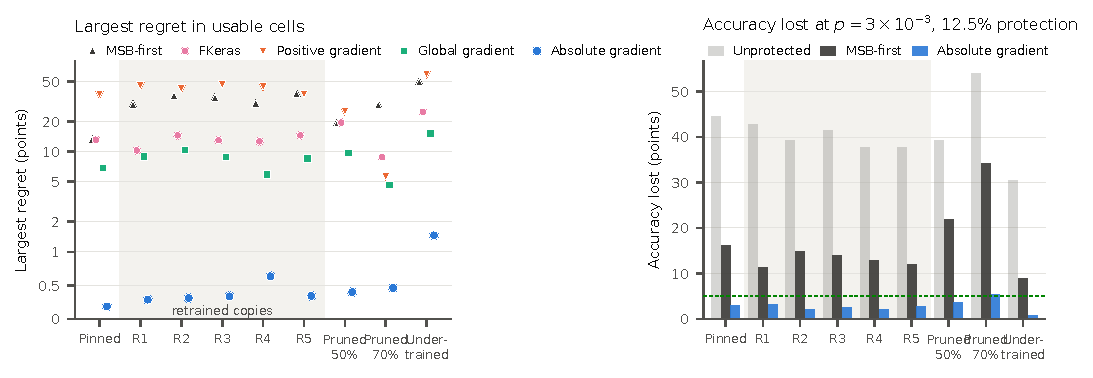
\includegraphics[width=\linewidth]{tecs_checkpoint_fragility}
\caption{The ResNet-8 checkpoints of Table~\ref{tab:repeated}: the pinned MLPerf reference, five copies retrained with its recipe (R1--R5), two pruned checkpoints and one under-trained checkpoint. Left: largest regret of each ranking in decision-useful cells (symmetric-log axis). Right: accuracy lost at $p=3\times10^{-3}$ and 12.5\% protection; the dashed line is the usefulness margin.}\label{fig:fragility}
\Description{Two panels comparing MSB-first, FKeras, gradient rankings and no protection across nine ResNet-8 checkpoints.}
\end{figure} These statements concern the seven rankings; search-based and literature-derived masks are compared in Section~\ref{sec:discussion}.

\subsection{When the preferred ranking changes}\label{sec:reversals}
The examples of Section~\ref{sec:allocation} show that the preferred ranking can depend on BER and budget. With masks built from 64 calibration inputs, this happens in the decision-useful region on the language models and on the under-trained ResNet-8; no pair of rankings shows resolved wins in both directions on the pinned or pruned ResNet-8, DS-CNN or ToyCar, and the single such pair on DistilBERT involves the random baseline. With more calibration inputs it happens on most ResNet-8 checkpoints.

On Pythia and Qwen the reversals are dominated by the positive-gradient ranking. It is the best measured ranking at the lowest BERs, by 0.01 to 0.03 nats per token over absolute gradient on Qwen at $p\le3\times10^{-4}$, and becomes worse by 0.2 to 1.1 nats per token at $3\times10^{-3}$ and by 3.8 at $10^{-2}$. What it gains where faults are sparse is two orders of magnitude smaller than what it loses where they are not.

On the under-trained ResNet-8 the same ranking produces a reversal that matters at both ends. At $p=10^{-3}$ the positive-gradient mask is better than the absolute-gradient mask by 1.3 accuracy points at 12.5\% protection (interval 1.0 to 1.7; 0.8 to 1.8 with the replication as the unit) and by 1.1 points at 25\%, both resolved after Holm correction. At $p=10^{-2}$ it is worse by 22.6 and 12.3 points. All four cells are decision-useful, so for this checkpoint no single static ranking is best across the useful band. At $10^{-3}$ the positive-gradient mask even leaves the model 1.2 points more accurate than it is without faults; Section~\ref{sec:harm} explains why.

The well-trained checkpoints hide the same reversal behind the calibration size (Appendix~\ref{app:calibration}). The positive score $\E_x\max(0,e_b)=\tfrac12(\E_x|e_b|+\E_x e_b)$ contains the mean effect $\E_x e_b$, whose per-input terms largely cancel, so 64 inputs estimate it poorly. With both masks built from 1,024 inputs, the positive-gradient mask is ahead at $10^{-3}$ in all 36 decision-useful cells of the nine checkpoints, by 0.2 to 1.6 points, and behind in all 15 at $10^{-2}$, by 0.6 to 17.8. Five checkpoints, the pinned one included, show resolved wins in both directions, and by the rule fixed before the runs the default does not hold at 512 or more inputs. Its own mask is settled at 64 inputs.

Two further effects are smaller: on Pythia at $p=3\times10^{-3}$ and 25\%, where it protects two complete tiers, MSB-first is better than absolute gradient by 0.09 nats per token, and within a half-protected tier structured fills beat a uniformly random one while FKeras does not beat storage order (Appendix~\ref{app:repeated}). Reversals outside the decision-useful region are not interpreted, and a bit-exact replay of every saved language-model field shows that the loss cap changes no conclusion in a decision-useful cell (Appendix~\ref{app:evidence}).

\subsection{Protection that is worse than none}\label{sec:harm}
Under ideal suppression a protected model receives a subset of the faults of the unprotected model, so it is tempting to assume that protection can only help. Figure~\ref{fig:harm} shows that it need not. With the positive-gradient mask, DistilBERT has a higher error rate than the unprotected model in six cells, by up to 6.0 points (interval 4.7 to 7.3, at $p=3\times10^{-2}$ and 6.25\%), and a higher loss in 17 of 32 cells; Pythia has a higher loss in eight cells, by up to 5.8 nats per token. Four of the DistilBERT accuracy cells are decision-useful: a designer who chose this ranking would have done worse than by protecting nothing, while the absolute-gradient mask keeps accuracy between 87\% and 90\% in the same cells. Checks for a defect in pairing, fault accounting, scores and nonfinite outputs found none (Appendix~\ref{app:harm}).

\begin{figure}[tbp]
\centering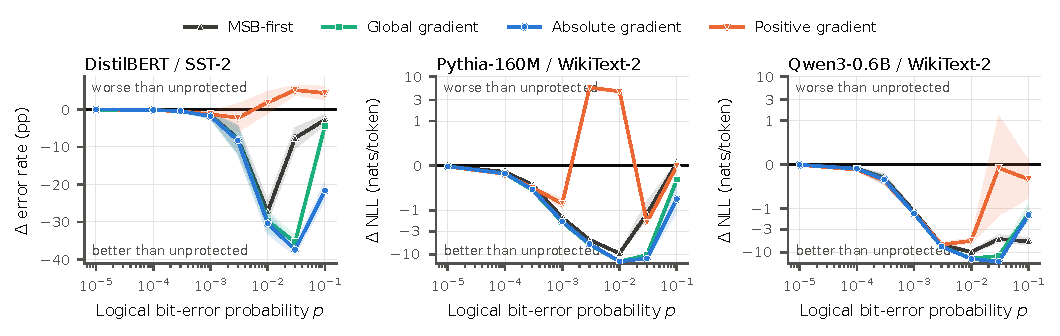
\includegraphics[width=\linewidth]{tecs_protection_vs_unprotected_125}
\caption{Paired difference between each protected model and the unprotected model on the same fault fields, at 12.5\% protection. Positive values mean protection made the task metric worse. Bands are 95\% paired intervals. The figure shows the three transformers, for which no FKeras ranking was measured.}\label{fig:harm}
\Description{Three panels showing that the positive-gradient mask becomes worse than no protection at intermediate bit-error probabilities.}
\end{figure}

The mechanism, obtained offline from the saved gradients, masks and stored codes of DistilBERT, is a one-sided remainder (Table~\ref{tab:drift} in Appendix~\ref{app:harm}). For every other mask the loss-increasing and loss-decreasing first-order effects of the unprotected bits cancel to within 0.5\%; the positive-gradient mask protects mainly loss-increasing flips, so the effects of what it leaves sum to $+6.7$ against $-20.6$. The many remaining faults then push the weights coherently in one direction, far beyond the range in which a gradient describes the loss. The amount of perturbation left is not the explanation: this mask leaves about the same squared jump size as the other gradient masks.

The under-trained ResNet-8 shows the same one-sided remainder with the opposite outcome at low fault rates. Its loss is not at a minimum, so a few faults pushed in the loss-decreasing direction act like a training step and raise accuracy above the clean model's; denser faults overshoot. A weaker form of this appears on the well-trained checkpoints once the positive score is estimated from more inputs (Appendix~\ref{app:calibration}). Its stored codes are distributed like those of the other checkpoints (Appendix~\ref{app:harm}), so the difference lies in where the weights sit on the loss surface, not in their values. Every ranking built from clean-model gradients assumes that the deployed model sits near a minimum, and a checkpoint that does not is one of the conditions under which a fixed ranking can mislead. The mechanism was checked directly for DistilBERT only.


\end{document}
